%% LyX 2.4.1 created this file.  For more info, see https://www.lyx.org/.
%% Do not edit unless you really know what you are doing.
\documentclass[english]{article}
\usepackage{lmodern}
\renewcommand{\familydefault}{\rmdefault}
\usepackage[T1]{fontenc}
\usepackage[latin9]{inputenc}
\synctex=-1
\usepackage{color}
\usepackage{babel}
\usepackage{float}
\usepackage{amssymb}
\usepackage{graphicx}
\usepackage{rotfloat}
\usepackage{setspace}
\usepackage[pdfusetitle,
 bookmarks=true,bookmarksnumbered=false,bookmarksopen=false,
 breaklinks=false,pdfborder={0 0 1},backref=false,colorlinks=true]
 {hyperref}

\makeatletter
%%%%%%%%%%%%%%%%%%%%%%%%%%%%%% User specified LaTeX commands.
%%base:
\usepackage{amsfonts}
\usepackage{setspace}
\usepackage{fullpage}
\usepackage{rotating}
\usepackage{booktabs}
\usepackage[abbr]{harvard}
\usepackage{color}

\renewcommand{\floatpagefraction}{.99}
\renewcommand{\topfraction}{.99}
\renewcommand{\bottomfraction}{.99}
\renewcommand{\textfraction}{0.01}

%%Cross reference figs and tabs
\AtBeginDocument{%
\let\ref\autoref
\renewcommand\figureautorefname{\@gobble}
\renewcommand\tableautorefname{\@gobble}
\renewcommand\equationautorefname{\@gobble}
}

\usepackage{color}
\hypersetup{colorlinks,linkcolor=blue}

\usepackage[toc,page]{appendix}



%%independence symbol
\newcommand\independent{\protect\mathpalette{\protect\independenT}{\perp}}
\def\independenT#1#2{\mathrel{\rlap{$#1#2$}\mkern2mu{#1#2}}}

%%or indep
\usepackage{graphicx}
\newcommand{\indep}{\rotatebox[origin=c]{90}{$\models$}}

%\usepackage[nolists,tablesfirst]{endfloat}
%\nomarkersintext

%\DeclareDelayedFloatFlavor{sidewaystable}{table}
%\DeclareDelayedFloatFlavor{sidewaysfigure}{figure}

\usepackage{graphicx,dblfloatfix}


% set hyperlink color
\usepackage{url}
\hypersetup{urlcolor=blue}

%%insert quote
\usepackage{epigraph}
\renewcommand{\textflush}{flushepinormal}
\setlength{\epigraphwidth}{0.9\textwidth}

% insert online Appendix: appendix page numbering
\let\origappendix\appendix % save the existing appendix command
\renewcommand\appendix{\clearpage\pagenumbering{roman}\origappendix}

% modify a page's margin e.g. abstract page
\usepackage{changepage}

%supress reference label/number

%change arabbic to roman numeral?
\renewcommand\thesection{\Roman{section}}
%\renewcommand\thesubsection{\Alph{subsection}}

%set some pages portrait?
\usepackage{pdflscape}


\usepackage[T1]{fontenc}

%stop table exceeding page
\usepackage{graphicx}

%include link in tex tables
\usepackage{url} 

%remove numbering of references
%\makeatletter
%\renewcommand\@biblabel[1]{}
%\makeatother

\usepackage{threeparttablex} % for footnote after longtable

\makeatother

\begin{document}
\thispagestyle{empty} \doublespace\begin{adjustwidth*}{+1.cm}{+1.cm}
\begin{center}
{\large\textbf{THE VALUE OF COMMUNICATION FOR MENTAL HEALTH}}{\large\vspace*{0.5cm}
\hspace{1cm}Francis Annan$^{\clubsuit}$ \hspace{4cm}Belinda Archibong$^{\spadesuit}$}\\
{\small University of California, Berkeley and NBER\hspace{1cm}Johns
Hopkins University SAIS and NBER}{\large}\\
\textbf{ OCTOBER 2024}
\par\end{center}

\end{adjustwidth*}\begin{adjustwidth*}{+1.1cm}{+1.1cm}{\large\vspace*{0.5cm}
}{\large\par}
\begin{center}
\textbf{Abstract}
\par\end{center}

\begin{onehalfspace}
\noindent Mental health disorders account for a significant share
of the overall global disease burden. The economic losses from such
disorders are staggeringly large, particularly in low-income countries,
where people are faced with several unexpected shocks. We test whether
improved communication can mitigate such mental health disorders.
Partnering with a major telecommunications company, we implement low-cost
communication interventions that provide mobile calling credits to
a nationally representative set of low-income adults in Ghana during
the COVID-19 pandemic. Individuals\textquoteright{} inability to make
unexpected calls, need to borrow SOS airtime, and to seek digital
loans decreased significantly relative to a control group. As a result,
the programs led to a significant decrease in mental distress (-9.8\%),
the likelihood of severe mental distress by -2.3 percentage points
(a quarter of the mean prevalence), and domestic violence, with null
impact on overall consumption expenditure. The effects are stronger
for monthly mobile credits than a lump-sum. We present evidence that
improvements in both business-related services and social inclusion
and/or protection are relevant explanations. Simple cost-benefit analysis
shows that providing communication credit to low-income adults is
a cost-effective policy for improving mental health. Communication
\textendash{} the ability to stay connected \textendash{} meaningfully
improves mental well-being and interventions about communication are
particularly valuable when implemented as many installments.
\end{onehalfspace}

\end{adjustwidth*}

\begin{doublespace}
\noindent{\large\textbf{K}}\textbf{EYWORDS}{\large\textbf{:}}{\large\textit{
Communication}}{\large{} (L63, O12), }{\large\textit{Well-being}}{\large{}
(I38), }{\large\textit{Mental Health and Domestic Violence}}{\large{}
(I12, I15)}{\large\par}
\end{doublespace}

\begin{singlespace}
\noindent\rule{0.3\columnwidth}{0.5pt}\\
$\clubsuit$ Corresponding Author: University of California, Berkeley,
207 Giannini Hall, Berkeley, CA 94720 and NBER. e-mail: \texttt{fannan@berkeley.edu}.
$^{\spadesuit}$ Johns Hopkins University SAIS, 555 Pennsylvania Avenue
NW, Washington DC 20001 and NBER. email: \texttt{barchib2@jh.edu}.
Field support from Samuel Adotevi, Kwamena Arkafra and Felix Debrah
(Ghana Statistical Service) and all field officers is acknowledged.
Jessica Moreira provided excellent research assistance. We thank Nathaniel
Hendren, Erzo F.P. Luttmer, Albert Ortega, David Cutler, Carol Graham,
AEA/ASSA 2021, Brookings, and NBER COVID-19 and Health Outcomes meeting
participants for comments on a draft of this paper. We are grateful
to three anonymous referees and the editor for their insightful comments.
We are grateful to the Columbia University CPRC and Earth Institute
for funding. The CPRC and Earth Institute had no involvement in any
substantive aspect of the research project. Institutional Review Board
(IRB) approvals for research data collection were obtained from Georgia
State University and Barnard College, Columbia University. The project
was registered in the AEA RCT Registry, AEARCTR-0006104.
\end{singlespace}

\pagenumbering{arabic} \doublespace 
\begin{onehalfspace}

\section{Introduction}
\end{onehalfspace}

\begin{doublespace}
\noindent{\large Imagine that you are unable to communicate \textendash{}
to make a phone call, use the web, access social media, and so on
\textendash{} when the need arises unexpectedly. Does this matter
for individuals' mental and economic well-being? Should communication
interventions during pandemics be applied as a one-time large transfer
or as numerous small installments? How valuable or cost-effective
is a policy that provides communication credit to low-income adults
for improving mental health? We use evidence from the COVID-19 pandemic
to address these important questions.}{\large\par}
\end{doublespace}

\begin{doublespace}
{\large Throughout the world, major communication interventions were
initiated in the public and private sectors in response to the COVID-19
pandemic. In the United States, ATT Inc. provided free 10GB of internet
data per month for 60 days as temporary relief for eligible customers
to enable them to stay connected during lockdown, starting March 27,
2020 (ATT Inc. 2020).}{\large\footnote{\noindent{\large As the leading provider of mobile services in the
US, with about 40\% share of the market, ATT Inc.'s initiative affected
a significant number of people, particularly those in the low-income
communities. Others telecommunications companies, such as Comcast
Corporation, have deployed similar interventions, providing essential
internet and mobile services without charge to low-income families,
including seniors, veterans, and people with disabilities (Comcast
Corp. 2020). We provide a global review of COVID-19-induced communication
programs in Tables \ref{fig:globalreviewp1} and \ref{fig:globalreviewp2}.}}}{\large{} In Ghana, the government reduced the Communication Service
Tax (CST) from 9\% to 5\%, which reflected a reduction in the cost
of mobile talk time and data purchases, effective from September 15,
2020, in response to the economic and social hardships induced by
the pandemic (Ghana Revenue Authority 2020; Figure \ref{fig:photo_comm_interventions}).
The need for such communication programs was particularly crucial
in developing countries where the informal sector is large and the
COVID-19 crisis presented a substantial threat to individuals who
face credit, savings, and psychological stressors and constraints
(Banerjee, Niehaus, and Suri 2019). Despite the increase in these
communication-based programs globally, there is relatively little
evidence on their impacts on well-being during a pandemic.}{\large\par}

{\large Administrative data on mobile financial transactions from a
major provider in Ghana sheds light on the potential value of communication
during the pandemic. Figure \ref{fig:mobileTransactions} shows the
distribution of transactions and illustrates that while the overall
market activity decreased following the onset of the pandemic, interestingly
and in contrast, the demand for mobile airtime-related activities
(as measured by the purchase of data and airtime amounts, and thus
their demand) sharply increased over the period. This descriptive
evidence documents the importance of communication during the pandemic
and is congruent with our baseline surveys: 68\% of individuals indicated
that their need to call or connect with others (family, friends, employers)
had increased due to the COVID-19 pandemic and its disruptions. Yet,
between 52\% and 62\% indicated that, sometimes, when the unexpected
need arises, they were not able to call or connect with their family
and friends due to the economic hardships associated with the pandemic.
Thus, programs that directly mitigate such binding communication barriers
will likely have a larger impact on individual and societal well-being.}{\large\par}

{\large We use a randomized controlled trial (RCT) to estimate the
impacts of a short-term ``mobile phone calling credit'' among a
nationally representative set of a sub-population of low-income households
in Ghana during the COVID-19 pandemic. We draw on an existing nationally
representative baseline frame (Ghana Living Standards Survey 7 {[}GLSS7{]}),
and focus on 1,131 low income individuals or households that are readily
reachable by phone, work in the informal sector, and are located in
the bottom 75th percentile of the income distribution. This sample
is low income, where income and psychological constraints (Mullainathan
and Shafir 2013; Ridley et al. 2020) can easily bind due to pandemic-induced
economic losses, and spans 193 districts across the country's historical
ten administrative regions.}{\large\par}

{\large We partner with a major local telecommunications company to
run our experiment by randomly assigning the 1,131 individuals to
two candidate communication programs: 40GHS (US\$7.0) lumpsum mobile
credit (376 individuals) versus 20GHS (US\$3.5) monthly installments
of mobile credit over two months (371 individuals) versus a control
program (384 individuals); and then measuring how these affect individuals'
ability to mitigate unexpected communication constraints during the
pandemic, with impacts on well-being, that is, mental health, domestic
violence, and consumption expenditures. The different programs about
communication provide a means of examining how communication programs
might be delivered: one-time large communication transfer versus numerous
small installments.}{\large\par}

{\large The pandemic uncovered a great deal of mental health crises
(World Health Organization 2022)}{\large\footnote{{\large\href{https://www.who.int/news/item/02-03-2022-covid-19-pandemic-triggers-25-increase-in-prevalence-of-anxiety-and-depression-worldwide}{https://www.who.int/news/item/02-03-2022-covid-19-pandemic-triggers-25-increase-in-prevalence-of-anxiety-and-depression-worldwide}}}}{\large{}
and increased domestic violence (Leslie and Wilson 2020; United Nations
2022)}{\large\footnote{{\large\href{https://www.unwomen.org/en/news/in-focus/in-focus-gender-equality-in-covid-19-response/violence-against-women-during-covid-19}{https://www.unwomen.org/en/news/in-focus/in-focus-gender-equality-in-covid-19-response/violence-against-women-during-covid-19}}}}{\large ,
which have potentially large short- and long-term impacts on human
capital development. Mental health disorders account for 13\% of the
overall global disease burden (Collins et al. 2011). The economic
and productivity losses from such disorders are significant, particularly
in low-income countries (Mathers, Fat, and Boerma 2008; Canavan et
al. 2013; Adhvaryu et al. 2019).}{\large\footnote{{\large Mathers, Fat, and Boerma (2008) estimate that depression generates
losses of 55.5 million disability-adjusted life-years in low and middle-income
countries. Canavan et al. (2013) estimate that the productivity loss
linked to mental illness is equivalent to 7\% of Ghana\textquoteright s
GDP \textendash{} our country of study.}}}{\large{} The direct economic impact of COVID-19 in these environments
was high and includes earnings and consumption shortfalls (Banerjee
et al. 2020), food insecurity (Laborde et al. 2020), among many other
meaningful negative impacts. }{\large\par}

{\large How might communication affect well-being? Conceptually, communication
is a network good and could turn on at least three interesting channels:
(i) improved business-related services (via professional networks),
(ii) improved social inclusion and/or protection (via social networks),
and (iii) improved informal insurance arrangements or consumption
insurance (via social networks). First, professional networks operate
in form of affected individuals being able to stay in touch with customers
and buy/sell with vendors to increase their revenues, which has a
positive impact on mental well-being (see e.g., Ridley et al. 2020
for a detailed review). Second, social inclusion (or reduced isolation)
operates in form of individuals being able to stay in touch with friends/family
who can provide them emotional support (Mullainathan and Shafir 2013;
Leslie and Wilson 2020), or serve as agents of social control and
protection to specifically reduce domestic violence by increasing
the cost of violence (� la Gelles 1983; Gelles and Straus 1979). Third,
in vulnerable periods such as COVID-19 related lockdowns, households
might have difficulty communicating with their informal insurance
networks (family, friends, etc.) and thus consumption risk-sharing
ability may suffer (Blumenstock, Eagle and Fafchamps 2016; Jack and
Suri 2016). The provision of mobile credit might alleviate that constraint.
Our interventions are designed to both relax communication constraints
and test their impact on mental health, domestic violence, and consumption
expenditures.}{\large\par}

{\large We first conduct three baseline survey waves prior to the deployment
of the communication interventions. After fielding the first round
of interventions (lumpsum and first installment), we conducted two
endline survey waves to track the various outcomes. Our final dataset
is unique due to its size and national representativeness, the expansive
set of outcomes, the administrative data on mobile financial transactions,
and 1$\times$3 random variations for communication at the individual
level. We find five set of results: }{\large\par}

{\large First, as a first stage, the interventions decreased unexpected
communication constraints significantly. That is, our experimental
interventions mitigate individuals' inability to meet unexpected communication
needs and stay connected (-37pp=-74\% for inability to make unexpected
calls, -22pp=-78\% for unexpected need to borrow airtime, and -3.5pp=-44\%
to seek digital loans). These effects are larger and more sustained
over time for the installment communication credit program compared
to the lumpsum credit.}{\large\par}

{\large Second, we find meaningful improvement in psychological well-being,
which is measured using the Kessler Psychological Distress Scale (K10)
and on domestic violence. Both mental distress and severe mental distress
decreased by -9.8\% and -2.3pp (=-24\%) relative to a control group,
respectively. The installment communication credit program had larger
and more sustainable effects compared to the lumpsum credit. Only
the installment program led to a significant decrease in the overall
likelihood of individuals threatening their partners by -6.3\% (but
with no impacts on the overall likelihood of individuals hitting their
partners \textendash{} our second measure of domestic violence).}{\large\par}

{\large Third, we find a null improvement in direct economic well-being.
The provision of communication credits can free up an individual's
resources that would otherwise have been allocated to communication
for other consumption expenses. The overall effect is, however, null
on total consumption, which is reassuring since the size and specificity
of our intervention were not large enough  to meaningfully change
consumption. Only the installment communication intervention increased
consumption expenditures, but the size is very small economically
and only in endline wave 2. }{\large\par}

{\large Fourth, what explains the estimated communication impacts?
We explore three alternative explanations: (i) improved business-related
services, (ii) improved social inclusion, and (iii) improved informal
risk-sharing or consumption insurance. We find strong empirical support
for improvements in both business-related services (increased business-related
income) and social inclusion/protection (reduced isolation), but not
for consumption insurance. Treated individuals reported a significant
increase in income (+9.0GHS per week overall) from business-related
services. Similarly, treated individuals were less likely to report
being emotionally- and socially-tired (-31\% for the lumpsum credit
group; -52\% for the installment credit group) but were also more
likely to stay at home during the pandemic. These show that improvements
in professional networks and social inclusion are relevant explanations.
We also examine heterogeneity in treatment effects along four dimensions:
poverty, informality, gender, and lockdown. The effects are indistinguishable
by gender but are larger for individuals that are very poor, in the
informal sector, and located inside areas which were previously in
lockdown. }{\large\par}

{\large Fifth, the marginal value of public funds (MVPF) (Hendren and
Sprung-Keyser 2020) for a policy that provides communication credit
to low-income adults is 2.04, suggesting that US\$1.0 of spending
on this communication credit policy delivers more than US\$1.0 in
benefits to its beneficiaries. We show robustness of the various findings
to the post-double selection LASSO estimation procedure (Belloni et
al. 2014), including adjustments for multiple testing (Romano and
Wolf 2005) and attrition (Lee 2009; Behaghel et al. 2015).}{\large\par}

{\large We contribute to three distinct literatures. First, there is
almost no work connecting mental health, domestic violence and economic
impacts of information and communications technology (ICT) (Jensen
2007). We offer short-run causal view of what communication does to
mental health and domestic violence, connecting ICT, domestic violence
and mental health. Allcott, Gentzkow, and Song (2022) examines how
habit formation and self-control problems explain the usage of social
media, which is different from the mental health and/or domestic violence
that we evaluate. More recently, Gawai (2023) documents that broadband
rollout reduces depression symptoms among older adults.}{\large\footnote{{\large Related, DiNardi et al. (2019) show that an increase in broadband
coverage increases the body weight (not mental health or domestic
voilence) among white women, while Donati et al. (2022) documents
the adverse mental health effect of broadband among the youth.}}}{\large{} The theory of social control developed in sociology and applied
to intimate partner violence (see e.g., Gelles 1983; Gelles and Straus
1979) predicts that societal controls and protection can increase
the perpetrator\textquoteright{} costs of domestic violence and reduce
its incidence. We implement a test that provides an empirical support
for the theory to explain our communication credit impacts. }{\large\par}

{\large Second is the economics literature on interpersonal transfers
following unexpected shocks in low-income countries. Previous work
have examined how households endogenously respond to non-covariate
shocks by sharing consumption-related resources (Townsend 1994; Blumenstock,
Eagle and Fafchamps 2016; Pulver 2009; Jack and Suri 2016). We look
at a fully-covariate and prolonged shock and randomized communication
transfers. }{\large\par}

{\large Third, we add to the growing research on mental health and
economic impacts of disease epidemics (Adhvaryu et al. 2019; Banerjee
et al. 2020; Archibong and Annan 2020). We cleanly isolate ICT and
document how to rely on it to mitigate the mental health impacts of
pandemics and unexpected hardships. Related literatures on psychiatry
and epidemiology emphasize how digital technology has the potential
to improve traditional psychiatry care and epidemiological outcomes.
Torous et al. (2021) provide a detailed review of this emerging field
of \textquotedblleft digital psychiatry\textquotedblright .}{\large\par}

{\large Our results have implications for policy. Mitigation of unexpected
pandemics can be a daunting task. Policymakers battle on various fronts:
tackling the spread of the pandemic while easing the potential welfare
impacts of the negative income shock and constraints on individuals.
Our programs relax binding communication constraints (individuals
inability to meet unexpected communication needs and to stay connected)
and allow us to provide the first experimental evidence on the impact
of communication interventions from a nationally representative set
of low-income individuals on overall well-being and gender relations
during pandemics. The provision of phone credit is a cost-effective
policy for improving mental health and a low-cost intervention to
encourage people to remain indoors during lockdown, helping to reduce
infection. Thus, our results add to the space of potentially resilient
policy initiatives aimed at tackling pandemics (mitigating their impacts). }{\large\par}

{\large We proceed as follows: In Section II, we describe the research
setting, experimental design and data. Section III presents our main
results. In Section IV, we examine how communication affects well-being
to derive our interpretation of the results and their implications
for welfare. We conclude the paper with Section V.}{\large\par}
\end{doublespace}

\section{Experiment: Setting and Design}
\begin{doublespace}

\subsection{A Brief Global Review: Communication Interventions}
\end{doublespace}

\begin{doublespace}
\noindent{\large Despite their prevalence, we are not aware of any
review that highlights COVID19-induced communication interventions.
We begin with a careful and ambitious (yet incomplete) global search
of communication-related initiatives that were introduced in response
to the COVID-19 pandemic. Details are shown in Tables \ref{fig:globalreviewp1}
and \ref{fig:globalreviewp2}. Our review shows that several communication
interventions in different forms and scales (spatial and temporal)
took place during the crisis. Despite their prevalence and potential
importance, there is poor evidence on the impacts of such programs
during the pandemic on individuals' economic and psychological well-being.}{\large\par}
\end{doublespace}
\begin{doublespace}

\subsection{Research Context}
\end{doublespace}

\begin{doublespace}
\noindent{\large Our study is set in Ghana. Mobile phone connection
penetration is very high: mobile cellular subscriptions were 134 per
100 people in 2019 (rising from 70 per 100 people in 2010), even among
the poor (World Bank 2020). We draw on an existing nationally representative
baseline frame (GLSS7) of households in Ghana, which is housed by
the implementer of our surveys (Ghana Statistical Service {[}GSS{]}).
We then focus on a sub-population of low-income households (i.e.,
individuals/households located in the bottom 75th percentile of the
income distribution). These are largely married (91\%) individuals
(household heads), with over 22\% poverty rates and have mobile phone
and connection access that is readily reachable by phone. Individuals
without mobile credit can still take in-coming calls.}{\large\par}
\end{doublespace}

\begin{doublespace}
{\large Similar to many countries, the pandemic in Ghana had economic
impacts well beyond its health impacts, due to the restrictions on
mobility and interactions that it triggered. Following the arrival
of the first COVID-19 case in Ghana (March 03, 2020), the President
Nana Akufo-Addo announced a lockdown in the two most economically
active regions (namely, the Greater Accra Metropolitan Area and the
Greater Kumasi Metropolitan Area) on March 30, which was later followed
by a nation-wide closing of all schools and a ban on other activities
and which extended to these affected regions.}{\large\par}

{\large People were advised to stay at home and were only permitted
to leave their homes for essential items such as food, medicine, and
water, or to visit the bank and public toilets. Intercity travel for
private and commercial purposes, except for essential goods and services,
was suspended. In terms of intracity travel, vehicles drivers were
obliged to reduce their number of passengers to observe social distancing.
The borders were closed to all but returning Ghanaians and foreign
nationals with Ghanaian residence permits, who were subject to a 14-day
mandatory quarantine}{\large\textit{ }}{\large if the returnees showed
symptoms of the virus. From April 20, 2020, the lockdown was removed
and some of the restrictions were relaxed, yet individuals continue
to battle with the persistent impacts of these restrictions and prevailing
uncertainties.}{\large\par}

{\large Individuals in our baseline surveys, conducted in September
2020, are much aware of the pandemic and its associated restrictions
on economic activities. Almost 100\% of individuals indicated being
aware of COVID-19 and the restrictions, and 79\% trust the government
and the media to provide accurate statistics (cases, deaths) of the
pandemic. Meanwhile, 68\% of individuals reported their need to call
or connect with others (family, friends, employers) has unexpectedly
increased, yet over 52-62\% were sometimes unable to connect as a
result of the pandemic and its hardships. This is meaningful as 77\%
of the respondents are self-employed, 18\% are located in previously
locked-down regions, and 80\% are involved either fully or partially
in the informal sector. Table \ref{tab:summary-baseSurvey-all} contains
more detailed summaries.}{\large\par}
\end{doublespace}
\begin{doublespace}

\subsection{Measurement of Key Outcomes}
\end{doublespace}

\begin{doublespace}
\noindent{\large We define the various outcome measures: communication
constraints-mitigation, mental health, domestic violence, and consumption
expenditures: Communication constraints-(un)mitigation measures the
incidence of \textquotedblleft (un)mitigated\textquotedblright{} mobile
calls and transfers \textendash{} asking whether individuals were
unexpectedly confronted with the need to call or connect with others
(family, friends, work) but unable to do so because they }{\large\textit{lacked}}{\large{}
enough communication resources to remedy the costs. Under such dire
and unexpected situations (as it was during the pandemic), individuals
either borrow airtime (i.e., in-kind SOS credit with a service charge
of 10\% and fully repayable once subscribers recharge their phone
accounts with an amount that is more than the outstanding SOS credit
amount) or seek digital loans (i.e., short-term digital but cashable
loans with an interest of 6.9\% over 30 days) from telecommunications
providers. Therefore, we measure communication constraints-(un)mitigation
also based on the incidence of borrowing airtime or seeking digital
loans due to unexpected circumstances to connect with others.}{\large\footnote{{\large Unexpected communication needs are plausibly random, with higher
potential for more distress compared to needs that are expected. There
is room to adjust or plan for expected needs. Thus, communication
is likely more valuable to individuals when faced with unexpected
needs because of the less room to adjust.}}}{\large\par}
\end{doublespace}

\begin{doublespace}
{\large Consumption expenditures are measured across food (inside and
outside home), utilities, personal care, education, health, and durables
(economic well-being). Mental health is measured by the incidence
of mental distress (using Kessler Psychological Distress Scale (K10))
(psychological well-being). K10 values can range from 0 (minimum)
to 50 (maximum), and values above 30 are classified as severe mental
distress (Adhvaryu et al. 2019). Gender relations reflect domestic
violence (DV) and specifically elicit from an individual whether he/she
either threatened or hit his/her partner (Banerjee et al. 2020).}{\large\footnote{{\large We pre-specified our three primary outcomes in the AEA RCT
registry (AEARCTR-0006104): (i) Information and communication-sharing
(value, as measured by: unmitigated calls); (ii) Expenditures on and
conditional transfers; and (iii) Mental health, happiness and gender
relations. Two other outcomes that are not used were pre-specified.
The experimental design: 2 treatments (lump-sum vs installments) and
1 control program, stratified by localities (or districts) was also
pre-specified. Without loss, we implemented monthly rather than pre-planned
weekly installments to ensure better administrative oversight in the
field.}}}{\large{} We take advantage of our short research instrument, which
is limited in space, to measure additional variables: individuals'
characteristics (poverty, age, gender, educational-level, occupation,
etc.), awareness and beliefs about COVID-19, COVID-19 impacts and
communication constraints. We adapted a recently developed shortcut
\textendash{} yet rigorous, inexpensive, simple and transparent \textendash{}
measure of poverty called the \textquotedblleft Simple Poverty Scorecard\textquotedblright{}
(Schreiner 2015; Annan JPEForthcoming). These variables are used to
test for randomization balance and explore heterogeneity in treatment
effects. Summary statistics of the various well-being measures are
contained in Table \ref{tab:summary-baseSurvey-all} and Figures \ref{fig:subjects_k10_base}
and \ref{fig:subjects_totconsump_base}. See the Appendix for specific
questions and possible responses to relevant select variables.}{\large\par}
\end{doublespace}
\begin{doublespace}

\subsection{Intervention and Timetable}
\end{doublespace}

\begin{doublespace}
\noindent{\large We evaluate the impacts of two communication programs:
lumpsum mobile credit versus installments of mobile credit. Our goal
was to mitigate binding communication constraints during the pandemic
that render (potentially marginal) individuals unable to connect with
others when the unexpected need arises. The timetable of baseline
and endline activities is displayed in Figure \ref{fig:dataCollection}.
We use the administrative (transaction-level) data to calculate the
50th (75th) percentile purchase for airtime and data combined over
the data period to be 188GHS (308GHS) per month. We set the total
value of our communication credit intervention for each individual
to 40GHS, that is, 21\% of the median monthly purchase, or equivalently,
13\% of the 75th percentile monthly purchase. We estimate this amount
as sufficient to cover the most basic unexpected communication needs
over a month or two. We first conduct three baseline survey waves
prior to the deployment of the communication interventions, which
include:}{\large\par}
\end{doublespace}
\begin{itemize}
\begin{doublespace}
\item {\large\textbf{Treatment program I (Lump-sum):}}{\large{} individuals
received 40GHS as mobile credit for one time (not discounted).}{\large\footnote{{\large At a monthly nominal discount rate of 1.16\% (i.e., an annual
rate of 14\% in Ghana, see: \href{https://www.bog.gov.gh/treasury-and-the-markets/interbank-interest-rates/}{https://www.bog.gov.gh/treasury-and-the-markets/interbank-interest-rates/}),
the net present value terms of the 20GHS installment transfers is
39.31GHS, which is around the 40GHS lumpsum transfer. Due to the short
period of time (i.e., one month interval between the two 20GHS installments),
we expect discounting to have little or no effect.}}}{\large\par}
\item {\large\textbf{Treatment program II (Installments):}}{\large{} 40GHS
was split into two and individuals received this as mobile credit
in installments (20GHS two times with a month interval between the
two).}{\large\par}
\item {\large\textbf{Control program:}}{\large{} individuals received no mobile
credit.}{\large\par}
\end{doublespace}
\end{itemize}
\begin{doublespace}
\noindent{\large The communication credit could be used to make a
phone call, transfer airtime, visit the web, or access other social
media services. After fielding the first round of interventions (lumpsum
and first installment), we conducted two endline survey waves (see
Figure \ref{fig:dataCollection}). As shown in Figure \ref{fig:dataCollection},
we started with }{\large\textit{n}}{\large =1,993 individuals reachable
by phone in baseline step 0 to arrive at }{\large\textit{n}}{\large =1,131
eligible and select individuals in baseline step 1.}{\large\par}
\end{doublespace}
\begin{doublespace}

\subsection{Treatment Assignment}
\end{doublespace}

\begin{doublespace}
\noindent{\large We use a 1x3 factorial design, randomizing a total
of 1,131 representative individuals into 3 experimental communication
programs: lumpsum mobile credit (376 individuals), installments of
mobile credit (371 individuals), and control program (384 individuals).
We stratified based on districts, and all misfits were resolved and
randomly assigned. The values of the two treatment programs are equal,
as specified above. We partnered with a major telecommunications company
to directly deliver the mobile credits. }{\large\par}
\end{doublespace}
\begin{doublespace}

\subsection{Balance and Validity of Design}
\end{doublespace}
\begin{doublespace}

\subsubsection{Balance}
\end{doublespace}

\begin{doublespace}
\noindent{\large We base our treatment analysis on a comparison of
individuals that received the communication treatments with those
who did not receive the treatments. Successful randomization of treatments,
and thus identification, requires that the assignments to treatments
(i.e., lumpsum credit versus installments credit) are independent
of any relevant individual-level statistics. To test that these individuals
are comparable, we run the regression:
\[
y_{id}=\alpha+\beta\mathbf{M}_{i}+\epsilon_{id}
\]
}{\large\par}

\noindent{\large on the baseline data (waves 1 and 2), where $\mathbf{M}_{i}=1$
if individual $i$ in district $d$ received a communication credit
treatment, and 0 otherwise. We consider the various treatments separately
and together (pooled) for a number of different outcomes and show
that individuals show no observable differences across the two groups.
Tables \ref{tab:treatment_balanceY} and \ref{tab:treatment_balanceXs}
report the pre-treatment balance results and provide strong evidence
in favor of randomization balance with no difference across individuals
in assigned (treated) and non-assigned (control) programs.}{\large\par}
\end{doublespace}
\begin{doublespace}

\subsubsection{Attrition}
\end{doublespace}

\begin{doublespace}
\noindent{\large Our randomization is based on the selected individuals
that draws on the baseline GLSS data files and step 0. Table \ref{tab:Attrition_summary}
displays the breakdown of response rates and attrition between baselines
and endlines. Here, attrition may be linked to individuals non-response
and inability to reach the participants either because their phone
numbers are inactive or out of network coverage area. To maximize
response rates, trained field officers conducted multiple phone calls
(see Figure \ref{fig:subjects_reachability}) at different time horizons
of the day, varying either weekdays or weekends, combined with step
0 that introduced the project and solicited the consent of the individuals.
If we aggregate all the data rounds, we record an overall attrition
rate of 6.5\%, which is low, given the uncertainty during the pandemic.
In our empirical estimations, we evaluate and formally show robustness
to attrition by treatment status.}{\large\par}
\end{doublespace}
\begin{doublespace}

\section{Experiment: Results}
\end{doublespace}

\begin{doublespace}
{\large We present and discuss the treatment effects. Since all our
treatments are about communication (or mobile calling) credit provision,
we first report the (combined) pooled effect of communication credit
assignment, and then the separate effects for the different treatments.}{\large\par}
\end{doublespace}
\begin{doublespace}

\subsection{Empirical Specifications}
\end{doublespace}

\begin{doublespace}
\noindent{\large We estimate treatment effects using the model:
\[
y_{idt}=\beta\mathbf{M}_{id}+\mathbf{X}_{id}^{\prime}\xi+\eta_{d}+\mu_{t}+\epsilon_{idt}
\]
 which links various outcome(s) $y_{idt}$ of individual $i$ in district
$d$ at date $t$ to the random treatment program(s) $\mathbf{M}_{id}$,
district-level (stratification unit) dummies $\eta_{d}$, date of
survey fixed effect $\mu_{t}$ (absorbs waves), and additional vector
of controls $\mathbf{X}_{id}$ which include the baseline outcomes.
For the pooled effects, $\mathbf{M}_{id}$ is a 0-1 indicator for
whether an individual received any of the communication programs,
and thus }{\large\textbf{$\beta$}}{\large{} captures the (pooled) treatment
effect. For the separate effects, $\mathbf{M}_{id}$ is a 0-1 indicator
for whether an individual received a specific communication program.
We denote by $\beta_{1}$ and $\beta_{2}$ the separate treatment
effects for lumpsum and installments programs, respectively (i.e.,
$\beta=(\beta_{1},\beta_{2})^{\prime}$). }{\large\par}
\end{doublespace}

\begin{doublespace}
{\large We take a theory-driven approach and use machine learning (specifically
LASSO) to select which out of the long list of controls $\mathbf{X}_{id}$
we should include. We do this using the post-double-selection LASSO
technique of Belloni et al. (2014). The post-double-selection LASSO
for estimating the impacts deals with potential covariate imbalance
(if any), and thus we can achieve good estimation performance, in
addition to minimizing researcher degrees of freedom and the possibility
for }{\large\textit{p}}{\large -hacking. For our main results, standard
errors are clustered at the individual level (the level of treatment)
to account for arbitrary correlations (Cameron and Miller 2015). Clustering
at district-level yields the same inference. To address the potential
issue of multiple testing, we adjust }{\large\textit{p}}{\large -values
for multiple testing across the family of outcomes following the procedure
presented in Romano and Wolf (2005). To evaluate and show robustness
for potential attrition bias, we report Lee (2009) attrition bounds
(trimming based on observed attrition rates; see Table \ref{tab:Attrition_summary}),
Imbens and Manski (2004) confidence sets, and Behaghel et al. (2015)
attrition bounds (trimming based on the number of times individuals
were called before answering the phone survey; see Figure \ref{fig:subjects_reachability}).}{\large\par}
\end{doublespace}
\begin{doublespace}

\subsection{Treatment Effects}
\end{doublespace}

\subsubsection{Communication \textendash{} Ability to Stay Connected}

\begin{doublespace}
{\large Do communication credit interventions matter for individuals
communication? We begin by asking whether the communication programs
mitigated individuals' communication constraints. Table \ref{tab:mitigate_pooled_meta}
shows the pooled treatments effect for alternative communication outcomes.
Relative to a control group, individuals inability to make unexpected
calls for the previous 7 days decreased (-37pp = -74\% of control
mean), inability to make unexpected calls due to COVID-19 decreased
(-17pp = -38\%), unexpected need to borrow SOS airtime decreased dramatically
(-22pp = -78\%), and seeking digital loans decreased (3.5pp = 44\%)
as a result of the communication programs. Table \ref{tab:mitigate_pooled_sep}
reports the separate treatment effects for each communication program.
The installment program produces significantly larger mitigation of
the communication constraints compared to the lumpsum (}{\large\textit{p}}{\large -values
< 0.01). }{\large\par}

{\large These results strongly confirm that the interventions mitigated
individuals' binding communication barriers during the pandemic period,
showing economically a large and statistically significant decrease
in individuals' inability to communicate and stay connected.}{\large\par}
\end{doublespace}

\subsubsection{Psychological and Economic Well-being}

\begin{doublespace}
{\large Do communication interventions matter for well-being? We next
evaluate how the communication programs impacted the various well-being
outcomes. Table \ref{tab:consump_pooled_meta} shows the pooled treatments
effect on consumption expenditures. Table \ref{tab:health_pooled_meta}
displays the pooled result for mental health (measured using the Kessler
Psychological Distress Scale (K10)) and domestic violence. We find
null effect on total expenditures, which is reassuring since the size
and specificity of our intervention were not large enough for it to
be plausible to find meaningful impacts on consumption. There are,
however, positive effects only for utilities and durables.}{\large\footnote{{\large We conducted sensitivity checks on the utilities and/or durables
consumption outcomes. First, to account for outliers, we trimmed these
individual consumption data at both the 1\% and 5\% levels. We find
that the results are still significant (i.e., qualitatively similar
to the untrimmed outcomes) but the effect sizes are much smaller.
For utilities, the coefficient in now +3.910GHS at the 1\% trimming
level and +1.166GHS at 5\% trimming level compared to our baseline
estimate of +4.819GHS in Table \ref{tab:consump_pooled_meta}. For
durables, the coefficient in now +5.077GHS at the 1\% trimming level
and +0.386GHS at 5\% trimming level compared to our baseline estimate
of +8.575GHS in Table \ref{tab:consump_pooled_meta}. Second, to weight
the tails of these individual consumption outcomes more, we rerun
the model using their log transformations (instead of their levels).
Here, we find that the results are very insignificant (}{\large\textit{p}}{\large -values
>0.36 in all cases). We conclude that the specific effects on utilities
and/or durables alone are inconclusive or indecisive. Ignoring these
sensitivity checks, however, our baseline results suggest that making
communication easier, as we do in the experiment, can raise the spending
on durables. This is particularly interesting and relevant for policy
because consumers can rely on their durable stock most of the time,
and as such durable spending only adjust infrequently.}}}{\large{} }{\large\par}

{\large In contrast to the null effect on consumption, we find meaningful
impacts on psychological well-being (Table \ref{tab:health_pooled_meta}):
mental health and domestic violence. Mental distress (measured by
$\log$K10) decreased by -9.8\%. Individuals were -6.3\% less likely
to threaten their partners relative to the control group (Romano-Wolf
}{\large\textit{p}}{\large -value=0.1247 which is only significant
at the 13\% level), but with no effect on the likelihood of hitting
their partners. Similarly, Table \ref{tab:consumpxhealth_pooled_sep}
reports the separate treatment effects, showing larger treatment effects
of the installment intervention on mental distress, severe mental
distress (measured by K10 values > 30), and on domestic violence measures.
Individuals in the installment credit are less likely (-2.3pp $\approx$
-24\%) to suffer the incidence of severe mental distress and -9.7\%
less likely to threaten their partners (Romano-Wolf }{\large\textit{p}}{\large -value=0.019
which is significant at conventional levels). There is limited effect
of the lumpsum credit on severe mental distress. For consumption,
the separate effects are null and indistinguishable across the two
communication treatments, which is not surprising because of the the
overall null pooled treatments effect on consumption expenditures
(see Table \ref{tab:consump_pooled_meta})}{\large\par}

{\large For potential dynamic effects, Figures \ref{fig:mitigate_trajectory_meta}-\ref{fig:consumpxhealth_trajectory_sep}
show the results over the trajectory survey by survey. What is significant
to note is that the installment program has larger and more sustainable
effects compared to the lumpsum, with the exception of consumption.
This may reflect either time inconsistency or social pressure problems
from receiving one-time large transfers.}{\large\par}
\end{doublespace}

\section{Interpreting the Results, Heterogeneity, and the Value of Communication}

\subsection{Interpreting the Results}

\begin{doublespace}
{\large How does communication affects well-being? We seek to understand
what happens when we give mobile credit to (potentially) }{\large\textit{communication-constrained}}{\large{}
individuals during unexpected hardships. Conceptually, communication
is a network good and could turn on at least three interesting alternative
interpretations: (i) improved business-related services (via professional
networks), (ii) improved social inclusion and/or protection (via social
networks), and (iii) improved informal risk-sharing or consumption
insurance (via social networks). We find strong empirical support
for improvements in both business-related services and social inclusion,
but not for informal insurance networks. We discuss and explore these
alternative explanations for the communication impacts. }{\large\par}

{\large Professional networks operate in form of affected individuals
being able to stay in touch with customers and buy/sell with vendors
to increase their revenues, which we know has a positive impact on
mental well-being (Ridley et al. 2020). To measure this, we asked
respondents about their total hours worked for income and the amount
they received from business income-related activities at endline.
Treated individuals reported (insignificant) increase in their hours
worked but a very significant increase in incomes (+9.0GHS per week
overall) from business-related services (Table \ref{tab:_channels?}).
This indicates that improvements in professional networks is a likely
explanation. }{\large\par}

{\large Social inclusion (reduced isolation) operates in form of individuals
being able to stay in touch with friends/family who can provide them
emotional (Mullainathan and Shafir 2013) and social support, or serve
as agents of social control and protection to specifically reduce
domestic violence by increasing the cost of violence (� la Gelles
1983; Gelles and Straus 1979). To measure this, we asked respondents
about whether they were emotionally- and socially-tired of staying
at home at endline. We find very significant evidence that treated
individuals were less likely to report being emotionally- and socially-tired
(-31\% for the lumpsum credit group; -52\% for the installment credit
group) but were also more likely to stay at home or seek shelter during
the pandemic (Table \ref{tab:_channels?}). This shows that improvements
in social inclusion is a meaningful, relevant explanation. }{\large\par}

{\large Communication credit can improve or rejuvenate informal insurance
arrangements. In vulnerable periods such as COVID-19 related lockdowns,
households might have difficulty communicating with their informal
insurance networks (family, friends) and thus consumption risk-sharing
ability may suffer (Blumenstock, Eagle and Fafchamps 2016; Jack and
Suri 2016). The provision of mobile credit might alleviate that constraint.
We take advantage of our individual-level panel data on consumption
to measure this using changes in consumption growth at endline. The
pandemic's lockdown was a negative consumption shock (see Figure \ref{fig:_consumpShock?}):
individuals located in lockdown areas show a large decrease in consumption
growth (median=-13\%; mean=-45\%) compared to those in non-lockdown
areas (median=-8\%; mean=-27\%). Yet, we do not find evidence for
an impact of mobile credit on the negative consumption effect of the
lockdown (Table \ref{tab:_channels?}). Our test on consumption insurance
here (which is similar to the one in Cochrane 1991) regresses consumption
growth against the negative consumption shock (ie., lockdown) combined
with mobile credit (i.e., communication intervention). This result
suggests that improvements in informal insurance networks, while plausible,
is unlikely at play. }{\large\par}

{\large Finally, we note that the two channels we find evidence for
\textendash i.e., improved business networks and social inclusion/protection
\textendash{} are also consistent with B�land et al. (2021) who used
the Canadian Perspective Survey Series during the COVID-19 pandemic
to document that concerns about both finances and maintaining social
ties are significantly related to concerns about family stress and
domestic violence. }{\large\par}
\end{doublespace}

\subsection{Heterogeneous Effects}

\begin{doublespace}
{\large The analyses so far assume that the effects of the communication
intervention are uniform. Here, examine heterogeneity in treatment
effects along four dimensions: (i) poverty, (ii) informality, (iii)
gender, and (iv) lockdown. The results are shown in Tables \ref{tab:wellbeingXpoverty_pooled_meta}-\ref{tab:wellbeingXlockeddown_pooled_meta}.
The decrease in domestic violence is more significant for the very
poor, while individuals in the informal sector experienced significantly
larger and better mental health improvements. Conversely, females
experienced slightly better mental health effects but this is not
statistically significant, while individuals located in previously
locked-down areas are more eager to re-allocate their budgets to more
consumption (specifically, to utilities and durables, as expected).
The latter reflects individuals who might still be battling the persistent
economic impacts of the COVID-driven lockdowns. }{\large\par}

{\large The results on gender differences in domestic violence and
mental health/stress are worth discussing. Table \ref{tab:wellbeingXfemale_pooled_meta}
indicates that females are about -12\% (=(-0.14/1.16)x100) relatively
less likely to hit their partner, but when combined with mobile credit,
there is no significant difference in hitting a partner by gender.
Similarly, when the mobile credits intervention is combined with mental
health, we see no significant differences by gender. From the raw
data and on a scale of 1 (never) to 4 (very often), men reported an
average score of 1.15 hitting their partners versus females who reported
an average score of 1.09 hitting their partners (}{\large\textit{p}}{\large -value=0.124
from a }{\large\textit{t}}{\large -test of their difference). Mental
health was equally high, with an average score of 14.47 for males
and 14.55 for females. (}{\large\textit{p}}{\large -value=0.124 from
a }{\large\textit{t}}{\large -test of their difference). These unconditional
means from the data are consistent with the coefficients on female
in Table \ref{tab:wellbeingXfemale_pooled_meta}. B�land et al. (2021)
show that stress and domestic violence were high during the pandemic
for both men and women, which is consistent with summary statistics
from our raw data. }{\large\par}

{\large We interpret the lack of gender differences in mental stress
or domestic violence when combined with mobile credits within the
lens our Framework on channels, suggesting that mobile credit, in
our context, either reduces isolation and increase the cost of hitting
your partner or allows you to stay in touch with your business clients,
thereby minimizing mental stress and the potential to hit your partner
if engaged in business activities. These results are in the right
direction, and thus reassuring and provide corroborative support for
our main findings.}{\large\par}
\end{doublespace}

\subsection{Discussions}

\begin{doublespace}
{\large We document the well-being impacts of providing low-cost in-kind
communication transfers. A natural question is }{\large\textit{how
does such in-kind transfers compare to cash transfers?}}{\large{} Our
experiments did not include a separate treatment program for cash,
but one can draw some insights from the ongoing large literature on
cash transfers during the pandemic (see e.g., Banerjee et al. 2020).
In rural Kenya, Banerjee et al. (2020) examined the effects of a Universal
Basic Income (UBI) during the COVID-19 pandemic using a large-scale
experiment, showing moderate to no improvements on mental health measures.
For context, their cash interventions transferred \$0.75 per day (amounting
to a non-discounted total of about \$23.3 per month) to the beneficiaries,
which is much larger than the cash equivalence of our in-kind communication
transfers, yet we find meaningful improvements on our mental health
measures. We do not find any impact on food consumption (Table \ref{tab:consump_pooled_meta})
and therefore no impact is likely to be found on hunger, but Banerjee
et al. (2020) reported modest UBI improvements on food consumption
(meat/fish) and hunger. Thus, it seems communication transfers might
yield larger improvements in mental health relative to cash transfers. }{\large\par}
\end{doublespace}

\subsection{The Value of Communication}

\begin{doublespace}
{\large To put our causal estimates into context, we consider the cost-effectiveness
of a policy that }{\large\textit{provides communication credit to
low-income adults for two months}}{\large . To compare the cost of
this policy that provides communication transfers with the associated
benefits, we adapt Hendren and Sprung-Keyser (2020)'s cost-benefit
framework that is conducive to empirical welfare analysis. Specifically,
we calculate the marginal value of public funds (MVPF), which estimates
the ratio of society\textquoteright s willingness to pay for the provision
of communication credit to the net cost to the government (here, an
``imagined'' funder) of implementing this policy. }{\large\par}

{\large We estimate society's willingness to pay (MVPF's numerator)
to include two main components. First, is the averted (otherwise)
social cost of mental health burden, $\xi$. We assume mental health
disorders account for 13\% of disease burden (Adhvaryu et al. 2019).
With a health expenditure per capita of US\$78 in Ghana (World Bank
2018), and a treatment effect of -10\% reduced mental destress rate,
we conservatively estimate the averted social cost of mental health
burden to be $\xi$ = 0.10x0.13xUS\$78=+US\$1.014. Our $\xi$ estimate
is very conservative in comparison to Addo et al. (2013) that would
have implied a +US\$2.68 averted social cost (2.6 times larger). Second,
is the individual beneficiary's willingness to pay for not visiting
the hospital or not getting mentally unwell, $\eta$, which includes
three sub-component estimates: (i) out-of-pocket health bill ($\eta_{1}$
=+US\$0.82); (ii) travel cost to health centers ($\eta_{2}$=+US\$0.203),
and (iii) lost income from missed work ($\eta_{3}$=+US\$11.55). Together,
the MVPF's numerator = $\xi$+$\sum_{i=1}^{3}\eta_{i}$=US\$13.590
for the average treated individual. We drop the direct value of the
communication subsidy to beneficiaries (+US\$7.0) to avoid double
counting. }{\large\par}

{\large Next, we estimate the net cost to the ``imagined'' funder
or government (MVPF's denominator) to include two main components.
First, is the cost of providing communication transfer for two months,
$G$ (=+US\$7.0). Second, is the missed communication services tax
(CST) revenue if individuals do not communicate or stay connected,
$\mu$. In Ghana, the CST is used to finance the National Youth Employment
Programme (NYEP) ($\geq$20\% of the CST) and support other national
development activities. Using the prevailing 5\% CST rate (Ghana Revenue
Authority 2020), we estimate that the government loses 0.05xUS\$7.0=
-US\$0.35. We intentionally over-estimate the total cost of this policy:
(i) communication is a network good so the ultimate economic incidence
of these communication transfers extends to other individuals \textendash{}
others might benefit from receiving mobile phone calls from the treated
individual (positive externalities). Arguably, such positive externalities
dominate the potential congestion hassle or traffic on the communication
network (negative externalities) (Bj�rkegren 2019 provides an example
in Rwanda). (ii) We conservatively did not factor in the reduced fiscal
cost from less hospital visits due to the reduced likelihood of mental
health disorders and/or domestic violence. Together, the MVPF's denominator
= $G$+$\mu$=US\$6.65 for the average treated individual.}{\large\par}

{\large Finally, taking the ratio, we estimate a conservative MVPF
of providing communication credit to be $\frac{13.590}{6.650}=2.044$.
This suggest that US\$1.0 of spending on this communication credit
policy delivers more than US\$1.0 in benefits to its beneficiaries.
Alternatively, the MVPF estimate implies that US\$1 of expenditure
yields US\$2 of total benefits, and so generates US\$1 of net benefits.
At the aggregate level, the policy's total benefit will be US\$54,035,343
against a total cost of US\$26,441,135. Notice that in determining
the MVPF, we intentionally bias the estimates to understate the benefits
and overstate the costs (Appendix section VI.8 contains additional
details).}{\large\par}
\end{doublespace}
\begin{doublespace}

\section{Conclusion}
\end{doublespace}

\begin{doublespace}
{\large The COVID-19 pandemic uncovered a great deal of economic and
mental health crises, most particularly for those people bound by
credit, savings and psychological constraints. This paper provides
new experimental evidence on the impact of providing communication
transfers. Communication during pandemics meaningfully matters for
well-being. Our mobile credit interventions led to a notable decrease
in unexpected communication constraints; individuals were better able
to mitigate their inability to meet unexpected communication needs
and stay connected. As a result, the programs led to meaningful well-being
improvements, particularly on mental health, but modestly on domestic
violence, and null on overall consumption expenditures. We present
evidence that improvements in both business-related services and social
inclusion/ protection are relevant channels explaining the estimated
communication impacts.}{\large\par}

{\large In terms of policy and design, communication initiatives that
relax potential communication constraints improve psychological well-being
and, to a modest degree, reduce domestic violence. However, these
programs are more valuable}{\large\textit{ }}{\large if implemented
in numerous installments of communication transfers, rather than one-time.
Simple cost-benefit analysis shows that providing communication credit
to low-income adults is a cost-effective policy for improving mental
health. There is almost no work linking mental health and information
and communications technology (ICT) (Jensen 2007; Blumenstock, Eagle
and Fafchamps 2016). We offer a short-run causal view of what communication
does to mental health, using evidence from an unexpected pandemic.}{\large\par}
\end{doublespace}
\begin{thebibliography}{10}
\begin{onehalfspace}
{\large\bibitem{key-18-1} Adhvaryu, Achyuta, James Fenske, and Anant
Nyshadham. 2019. ``Early Life Circumstance and Adult Mental Health.''
}{\large\textit{Journal of Political Economy}}{\large , 127(4): 1516-1549. }{\large\par}

\bibitem{key-6}{\large Addo, Rebecca, Justice Nonvignon, and Moses
Aikins. 2019. ``Household Costs of Mental Health Care in Ghana.''
}{\large\textit{J Ment Health Policy Econ}}{\large , 16(4): 151-159. }{\large\par}

{\large\bibitem{key-4}Allcott, Hunt, Matthew Gentzkow, and Lena Song.
2022. ``Digital Addiction.'' }{\large\textit{American Economic Review}}{\large ,
112 (7): 2424-63.}{\large\par}

{\large\bibitem{key-18}Annan, Francis. (Forthcoming). \textquotedblleft Misconduct
and Reputation under Imperfect Information. `` Journal of Political
Economy.}{\large\par}

\bibitem{key-1}{\large{} Archibong, Belinda and Francis Annan. 2020.
\textquotedblleft Schooling in Sickness and in Health: The Effects
of Epidemic Disease on Gender Inequality. `` Working Paper, UC Berkeley.}{\large\par}

\bibitem{key-12}{\large{} Banerjee, Abhijit, Michael Faye, Alan Krueger,
Paul Niehaus, and Tavneet Suri. 2020. ``Effects of a Universal Basic
Income during the Pandemic.'' Working paper, UC San Diego.}{\large\par}

\bibitem{key-11}{\large{} Banerjee, Abhijit, Paul Niehaus, and Tavneet
Suri. 2019. ``Universal Basic Income in the Developing World.''
}{\large\textit{Annual Review of Economics}}{\large , 11(): 959-983. }{\large\par}

\bibitem{key-1}{\large{} B�land, Louis-Philippe, Abel Brodeur, Joanne
Haddad, and Derek Mikola. 2021. \textquotedblleft Determinants of
Family Stress and Domestic Violence: Lessons from the COVID-19 Outbreak\textquotedblright .
}{\large\textit{Can Public Policy}}{\large , 47(3): 439\textendash 459.}{\large\par}

\bibitem{key-2}{\large{} Behaghel, Luc, Bruno Crepon, Marc Gurgand,
and Thomas Le Barbanchon. 2015. \textquotedblleft Please Call Again:
Correcting Non-Response Bias in Treatment Effect Models.\textquotedblright{}
}{\large\textit{Review of Economics and Statistics}}{\large , 97(5):
1070-1080.}{\large\par}

\bibitem{key-6}{\large{} Belloni Alexandre, Victor Chernozhukov, and
Christian Hansen. 2014. ``Inference on Treatment Effects after Selection
among High-Dimensional Controls.'' }{\large\textit{Review of Economic
Studies}}{\large , 81(2): 608-650.}{\large\par}

\bibitem{key-8}{\large{} Blumenstock, Joshua, Nathan Eagle, and Marcel
Fafchamps. 2016. \textquotedblleft Airtime Transfers and Mobile Communications:
Evidence in the Aftermath of a Natural Disaster.\textquotedblright{}
}{\large\textit{Journal of Development Economics}}{\large , 120(C):
157-181. }{\large\par}

\bibitem{key-4} {\large Bj�rkegren, Daniel. 2019. ``The Adoption
of Network Goods: Evidence from the Spread of Mobile Phones in Rwanda.''
}{\large\textit{Review of Economic Studies}}{\large , 86(3): 1033-1060.}{\large\par}

\bibitem{key-4}{\large{} Cameron, Colin A. and Douglas L. Miller. 2015.
``A Practitioner's Guide to Cluster-Robust Inference.'' }{\large\textit{Journal
of Human Resources}}{\large , 50 (2): 317-373. }{\large\par}

\bibitem{key-9} {\large Canavan, M. E., H. L. Sipsma, A. Adhvaryu,
et al. 2013. \textquotedblleft Psychological Distress in Ghana: Associations
with Employment and Lost Productivity.\textquotedblright{} }{\large\textit{Interknits
J. Mental Health Systems 7}}{\large{} (1): art. 9.}{\large\par}

\bibitem{key-1} {\large Cochrane, H. John. 1991. ``A Simple Test
of Consumption Insurance.'' }{\large\textit{Journal of Political
Economy}}{\large , 99(5): 957-976. }{\large\par}

\bibitem{key-3}{\large{} Collins, Y. Pamela, Vikram Patel, Sarah S.
Joestl, et al. 2011. \textquotedblleft Grand Challenges in Global
Mental Health.\textquotedblright{} }{\large\textit{Nature}}{\large ,
475 (7354): 27-30. }{\large\par}

\bibitem{key-3}{\large{} DiNardi, M., Guldi, M. and Simon, D. 2019.
\textquotedblleft Body Weight and Internet Access: Evidence from the
Rollout of Broadband Providers.\textquotedblright{} }{\large\textit{Journal
of Population Economics}}{\large , 32, 877\textendash 913. }{\large\par}

\bibitem{key-4}{\large{} Donati, D., Sobbrio, F., Durante, R. and Zejcirovic,
D. 2022. ``Lost in the Net? Broadband Internet and Youth Mental Health.''
Working paper.}{\large\par}

\bibitem{key-2}{\large{} Gawai, Vikas PD. 2023. \textquotedblleft Does
High-Speed Internet Access Affect the Mental Health of Older Adults?\textquotedblright{}
Working paper.}{\large\par}

\bibitem{key-2}{\large{} Gelles, R. J. 1983. ``An Exchange/Social
Control Theory.'' The Dark Side of Families: Current Family Violence
Research pp. 151\textendash 165.}{\large\par}

\bibitem{key-1}{\large{} Gelles, R. J. and Straus, M. 1979. ``Determinants
of Violence in the Family: Toward a Theoretical Integration. `` In:
Burr, W.R., Hill, R., Nye, F.I. and R.I.L., Eds., Contemporary Theories
about the Family, Free Press, New York, 550-581.}{\large\par}

\bibitem{key-8}{\large{} Ghana Revenue Authority. GRA. 2020. https://gra.gov.gh/domestic-tax/tax-types/communication-service-tax/}{\large\par}

\bibitem{key-8} {\large Ghana Statistical Service. 2019. Ghana Living
Standards Survey (GLSS) 7. Main Report. Available here: https://www.statsghana.gov.gh/gssmain/fileUpload/pressrelease/GLSS7\%20MAIN\%20REPORT\_FINAL.pdf}{\large\par}

\bibitem{key-5}{\large{} Hendren, Nathaniel and Ben Sprung-Keyser.
2020. ``A Unified Welfare Analysis of Government Policies.''}{\large\textit{
Quarterly Journal of Economics}}{\large , 135(3): 1209-1318.}{\large\par}

\bibitem{key-50}{\large{} Imbens, Guido and Charles Manski. 2004. ``Confidence
Intervals for Partially Identified Parameters.'' }{\large\textit{Econometrica}}{\large ,
72(6): 1845-1857. }{\large\par}

\bibitem{key-12}{\large{} Jack, William and Tavneet Suri. 2016. ``The
Long-run Poverty and Gender Impacts of Mobile Money.\textquotedblright{}
}{\large\textit{Science}}{\large , 354 (6317), 1288-1292.}{\large\par}

\bibitem{key-7} {\large Jensen, Robert. 2007. \textquotedblleft The
Digital Provide: Information (Technology), Market Performance, and
Welfare in the South Indian Fisheries Sector.\textquotedblright{}
}{\large\textit{Quarterly Journal of Economics}}{\large , 122(3), 879-924.}{\large\par}

\bibitem{key-4-1}{\large{} Laborde, David, Will Martin, Johan Swinnen,
and Rob Vos. 2011. \textquotedblleft COVID-19 Risks to Global Food
Security.\textquotedblright{} }{\large\textit{Science}}{\large , 369
(6503): 500-502.}{\large\par}

\bibitem{key-3-1}{\large{} Lee, David. 2009. ``Training, Wages, and
Sample Selection: Estimating Sharp Bounds on Treatment Effects.''
}{\large\textit{Review of Economics Studies}}{\large , 76(3): 1071-1102. }{\large\par}

\bibitem{key-7} {\large Leslie, Emily and Riley Wilson. 2020. ``Sheltering
in Place and Domestic Violence: Evidence from Calls for Service During
COVID-19.'' }{\large\textit{Journal of Public Economics}}{\large ,
189(104241).}{\large\par}

\bibitem{key-2}{\large{} Mathers, C. D., D. M. Fat, and J. Boerma.
2008. The Global Burden of Disease: 2004 Update. Geneva: World Health
Org. }{\large\par}

\bibitem{key-10} {\large Mullainathan, Sendhil and Eldar Shafir. 2013.
}{\large\textit{Scarcity: Why Having Too Little Means So Much}}{\large ,
Time Books, Henry Holt and Company LLC. }{\large\par}

\bibitem{key-6}{\large{} Piquero, Alex R. , Jordan R. Riddell, Stephen
A. Bishopp, Chelsey Narvey, Joan A. Reid, and Nicole Leeper Piquero.
2020. ``Staying Home, Staying Safe? A Short-Term Analysis of COVID-19
on Dallas Domestic Violence.'' }{\large\textit{American Journal of
Criminal Justice}}{\large , 45: 601\textendash 635.}{\large\par}

\bibitem{key-10} {\large Pulver, Caroline. 2009. \textquotedblleft The
Performance and Impact of MPESA: Preliminary Evidence from a Household
Survey.\textquotedblright{} }{\large\textit{Presentation to FSD-Kenya}}{\large . }{\large\par}

\bibitem{key-3}{\large{} Ridley, Matthew W. , Gautam Rao, Frank Schilbach,
and Vikram H. Patel. 2020. ``Poverty, Depression, and Anxiety: Causal
Evidence and Mechanisms.'' }{\large\textit{Science,}}{\large{} 370(6522):
94-108.}{\large\par}

\bibitem{key-1}{\large{} Romano, Joseph P., and Michael Wolf. 2005.
``Exact and Approximate Stepdown Methods for Multiple Hypothesis
Testing.'' }{\large\textit{Journal of the American Statistical Association}}{\large{}
100(469): 94-108.}{\large\par}

\bibitem{key-6}{\large{} Schreiner, Mark. 2015. \textquotedblleft Simple
Poverty Scorecard-{}-Poverty-Assessment Tool for Ghana.\textquotedblright{}
Available here: http://www.simplepovertyscorecard.com/GHA\_2012\_ENG.pdf. }{\large\par}

\bibitem{key-1}{\large{} Torous et al. (2021). \textquotedblleft The
Growing Field of Digital Psychiatry: Current Evidence and the Future
of Apps, Social Media, Chatbots, and Virtual Reality.\textquotedblright{}
}{\large\textit{World Psychiatry}}{\large , 20(3): 318\textendash 335.
DOI: 10.1002/wps.20883}{\large\par}

\bibitem{key-3} {\large Townsend, M. Robert. 1994. ``Risk and Insurance
in Village India.'' }{\large\textit{Econometrica}}{\large{} 62(3):
539-591.}{\large\par}

\bibitem{key-14}{\large{} World Bank. 2018. ``World Development Indicators''.
Available here: https://data.worldbank.org/indicator/SH.XPD.CHEX.PC.CD?locations=GH }{\large\par}

\bibitem{key-5}{\large World Bank. 2020. ``World Development Indicators''.
Available here: https://data.worldbank.org/indicator/IT.CEL.SETS.P2?locations=GH}{\large\par}
\end{onehalfspace}

\end{thebibliography}

\section*{Main Results for Text}

\begin{landscape}
\begin{center}
{\large{}
\begin{figure}[H]
{\large\caption{\textbf{D}{\footnotesize\textbf{ATA COLLECTION AND TIMETABLE }}{\scriptsize\textbf{\protect\label{fig:dataCollection}}}}
}{\large\par}
\begin{centering}
{\large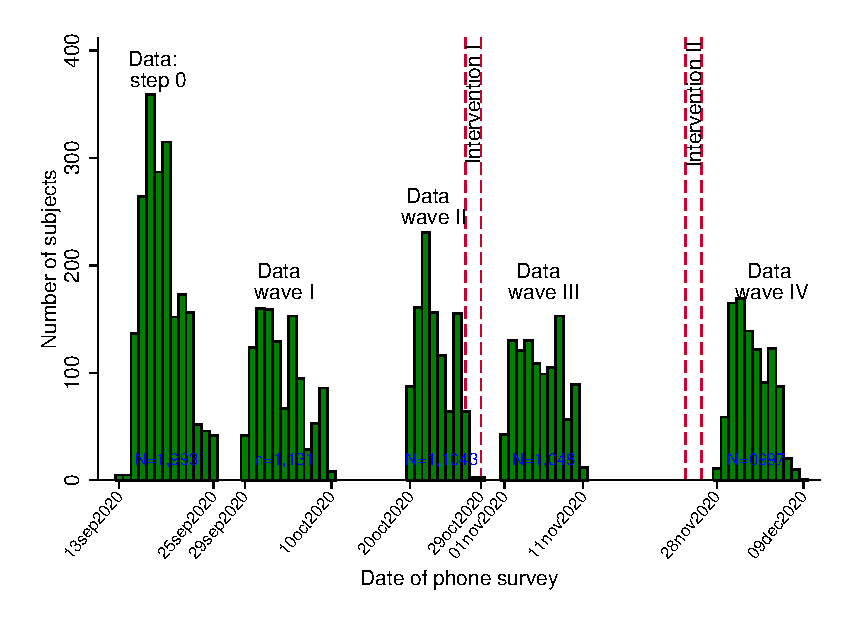
\includegraphics[scale=1.2]{../3-replication-package/original_figures/datacollectionr}}{\large\par}
\par\end{centering}
\begin{singlespace}
Note: Figure shows the timetable of baseline and endline data collection
activities. The various bars reflect the daily number of phone calls
or individuals surveyed. The baseline involves three panel survey
waves (step 0, wave I and wave II). These waves provide information
to determine eligible individuals and to conduct pre-intervention
randomization balance tests. The endline involves two panel waves
(wave III and wave IV) that follow the first round of interventions
deployment (Intervention I). Intervention I (the lumpsum and the first
tranche of credit installment) spans October 27-29, 2020. Intervention
II (the second tranche of credit installment) spans November 24-26,
2020. A lockdown was announced on March 30, 2020 and removed on April
20, 2020. The cumulative number of confirmed COVID-19 cases in Ghana
as of September 13, 2020 (the start of our experiment) was 45,434.
This increased to around 52,738 as of December 9, 2020 (the end of
our experiment). \href{https://www.statista.com/statistics/1110892/coronavirus-cumulative-cases-in-ghana/}{https://www.statista.com/statistics/1110892/coronavirus-cumulative-cases-in-ghana/}
\end{singlespace}
\end{figure}
}{\large\par}
\par\end{center}

\begin{center}
{\large{}
\begin{table}[H]
{\large\caption{\textbf{A}{\footnotesize\textbf{TTRITION}}{\large\textbf{ }}{\footnotesize\textbf{\protect\label{tab:Attrition_summary}}}}
}{\large\par}

\begin{ThreePartTable}
\begin{table}[tbp]\centering
\def\sym#1{\ifmmode^{#1}\else\(^{#1}\)\fi}
\caption{Attrition}
\begin{tabular}{lccccc}
\hline
 & Lumpsum & Installments & Control & Total & Attrition \\
\hline\hline
STEP 0  &                       &                 & 1,993 &                \\
*Verify phone numbers & & & & & \\ 
*Measure poverty (Schreiner 2005) & & & & & \\ 
SELECT SAMPLE (Randomized) & 376                &       371            &       384             &       1131          &                                       \\
BASELINE I (Wave 1)                 & 376               &       371            &       384             &       1131          &       0     \\
                                                    & (100\%)  &       (100\%)       &       (100\%)        &       (100\%) &   (0\%) \\
                                                    & (0\%)    &       (0\%)         &       (0\%)          &       (0\%)       &       (0\%)  \\
BASELINE II (Wave 2)        & 352               &       340            &       351             &       1043          &       88     \\
                                                    & (94\%)  &       (92\%)       &       (91\%)        &       (92\%) &   (8\%) \\
                                                    & (24\%)    &       (28\%)         &       (28\%)          &       (27\%)       &       (27\%)  \\
ENDLINE I (Follow-up wave 3) & 355              &       344            &       349             &       1048          &       83     \\
                                                    & (94\%)  &       (93\%)       &       (91\%)        &       (93\%) &   (7\%) \\
                                                    & (23\%)    &       (26\%)         &       (29\%)          &       (26\%)       &       (26\%)  \\
ENDLINE II (Follow-up wave 4) & 343             &       335            &       319             &       997          &       134     \\
                                                    & (91\%)  &       (90\%)       &       (83\%)        &       (88\%) &   (12\%) \\
                                                    & (28\%)    &       (30\%)         &       (38\%)          &       (32\%)       &       (32\%)  \\
\hline\hline
\end{tabular}
\end{table}


\begin{spacing}{0.8}
Note: Table reports the summary statistics for the subsample that
was successfully reached for a follow-up and for the subsample that
was not successfully reached in endline phone surveys. Shown for all
panel waves.
\end{spacing}
\end{table}
}{\large{} }{\large\par}
\par\end{center}

\begin{center}
\begin{table}[!tph]
\caption{\textbf{M}{\footnotesize\textbf{ITIGATION OF COMMUNICATION CONSTRAINTS
\protect\label{tab:mitigate_pooled_meta}}}}

\documentclass[]{article}
\setlength{\pdfpagewidth}{8.5in} \setlength{\pdfpageheight}{11in}
\begin{document}
\begin{tabular}{lcccccccc}
\multicolumn{9}{c}{Mitigation of communication constraints - unsaturated} \\ \hline
 & (1) & (2) & (3) & (4) & (5) & (6) & (7) & (8) \\
VARIABLES & unableCall7days1 & unableCall7days1 & unableToCOVID1 & unableToCOVID1 & digitborrow1 & digitborrow1 & digitloan1 & digitloan1 \\ \hline
 &  &  &  &  &  &  &  &  \\
tmt\_all & -0.0254 & -0.0135 & 0.00367 & 0.0236 & 0.00979 & 0.0172 & 0.00905 & 0.00518 \\
 & (0.0247) & (0.0220) & (0.0241) & (0.0214) & (0.0172) & (0.0164) & (0.0107) & (0.0105) \\
Constant & 0.265*** & 0.0109 & 0.319*** & 0.105 & 0.130*** & 0.202 & 0.0507*** & -0.0394*** \\
 & (0.0190) & (0.0692) & (0.0205) & (0.119) & (0.0132) & (0.142) & (0.0110) & (0.0129) \\
 &  &  &  &  &  &  &  &  \\
Observations & 2,045 & 2,018 & 2,045 & 2,018 & 2,045 & 2,018 & 2,045 & 2,018 \\
R-squared & 0.001 &  & 0.000 &  & 0.000 &  & 0.000 &  \\
District FE & No & Yes & No & Yes & No & Yes & No & Yes \\
Date FE & No & Yes & No & Yes & No & Yes & No & Yes \\
Controls & None & Post-Double LASSO & None & Post-Double LASSO & None & Post-Double LASSO & None & Post-Double LASSO \\
Mean of dep. variable & .2652173913043478 & .2652173913043478 & .3188405797101449 & .3188405797101449 & .1304347826086956 & .1304347826086956 & .0507246376811594 & .0507246376811594 \\
 Number of groups &  & 0 &  & 0 &  & 0 &  & 0 \\ \hline
\multicolumn{9}{c}{ Robust standard errors in parentheses} \\
\multicolumn{9}{c}{ *** p$<$0.01, ** p$<$0.05, * p$<$0.1} \\
\end{tabular}
\end{document}


{\large\vspace*{0.2cm}
}Note: District is the randomization strata. The double-post LASSO
specification considers all individual controls, and individual district
and survey date fixed effects in the possible control set. Controls
include: individual\textquoteright s age, 0-1 indicator for whether
married or not, 0-1 indicator for whether belongs to akan ethnic group
or not, 0-1 indicator for whether self employed or not, household
size, 0-1 indicator for whether operates in the informal sector, monthly
personal income over an ordinal scale of 1 to 5, 0-1 indicator for
whether attained junior high school (JHS) education, and individual\textquoteright s
gender. Observations are at the individual $\times$ date level. Clustered
standard errors (at the individual level; the level of treatment)
are reported in parentheses. {*}{*}{*} p<0.01 (1\% level), {*}{*}
p<0.05 (5\% level), {*} p<0.1 (10\% level). 90\% confidence sets (CS)
around attrition bounds are reported in brackets. Romano-Wolf multiple
hypothesis correction \textit{p}-values (Romano and Wolf {[}2005{]})
reported for communication outcomes family (Unable to Call, 7days
0-1; Unable to Call, COVID19 0-1; Borrow SOS Airtime 0-1; Seek Digital
Loan 0-1). Behaghel et al. (2015) attrition bounds (not reported)
are tighter.
\end{table}
\par\end{center}

\begin{center}
\begin{table}[!tph]
\caption{\textbf{M}{\footnotesize\textbf{ITIGATION OF COMMUNICATION CONSTRAINTS
\protect\label{tab:mitigate_pooled_sep}}}}

\begin{tabular}{lcccc} \hline
 & (1) & (2) & (3) & (4) \\
 & Unable to Call & Unable to Call &  &  \\
VARIABLES & 7days 0-1 & COVID19 0-1 & Borrow SOS Airtime 0-1 & Seek Digital Loan 0-1 \\ \hline
 &  &  &  &  \\
Lumpsum Credit ($\beta_1$) & -0.280*** & -0.119*** & -0.183*** & -0.0237* \\
 & (0.0239) & (0.0244) & (0.0200) & (0.0134) \\
Installments Credit ($\beta_2$) & -0.439*** & -0.225*** & -0.266*** & -0.0461*** \\
 & (0.0225) & (0.0240) & (0.0191) & (0.0131) \\
 &  &  &  &  \\
Observations & 2,019 & 2,019 & 2,019 & 2,019 \\
Number of groups & 0 & 0 & 0 & 0 \\
District FE & Yes & Yes & Yes & Yes \\
Date FE & Yes & Yes & Yes & Yes \\
Controls & PD LASSO & PD LASSO & PD LASSO & PD LASSO \\
Mean of dep. variable & 0.499 & 0.452 & 0.289 & 0.079 \\
p-value for test: $\beta_1$ = $\beta_2$ & 0.000 & 0.000 & 0.000 & 0.002 \\
Lee 2009 Attrition Bounds $\beta_1$ & [-0.108; -0.069] & [-0.038; 0.001] & [-0.089; -0.049] & [-0.034; 0.005] \\
Lee 2009 Attrition Bounds $\beta_2$ & [-0.310; -0.289] & [-0.198; -0.177] & [-0.190; -0.169] & [-0.057; -0.036] \\
Imbens-Manski 2004 CS $\beta_1$ & [-0.138; -0.043] & [-0.070; 0.030] & [-0.114; -0.030] & [-0.056; 0.020] \\
Imbens-Manski 2004 CS $\beta_2$ & [-0.338; -0.268] & [-0.230; -0.149] & [-0.215; -0.153] & [-0.079; -0.023] \\
p-value: Romano-Wolf Correction $\beta_1$ & 0.091 & 0.091 & 0.091 & 0.091 \\
 p-value: Romano-Wolf Correction $\beta_2$ & 0.091 & 0.091 & 0.091 & 0.091 \\ \hline
\end{tabular}


{\large\vspace*{0.2cm}
}Note: District is the randomization strata. The double-post LASSO
specification considers all individual controls, and individual district
and survey date fixed effects in the possible control set. Controls
include: individual\textquoteright s age, 0-1 indicator for whether
married or not, 0-1 indicator for whether belongs to akan ethnic group
or not, 0-1 indicator for whether self employed or not, household
size, 0-1 indicator for whether operates in the informal sector, monthly
personal income over an ordinal scale of 1 to 5, 0-1 indicator for
whether attained junior high school (JHS) education, and individual\textquoteright s
gender. Observations are at the subject $\times$ date level. Clustered
standard errors (at the individual level; the level of treatment)
are reported in parentheses. {*}{*}{*} p<0.01 (1\% level), {*}{*}
p<0.05 (5\% level), {*} p<0.1 (10\% level). 90\% confidence sets (CS)
around attrition bounds are reported in brackets. Romano-Wolf multiple
hypothesis correction \textit{p}-values (Romano and Wolf {[}2005{]})
reported for communication outcomes family (Unable to Call, 7days
0-1; Unable to Call, COVID19 0-1; Borrow SOS Airtime 0-1; Seek Digital
Loan 0-1). Behaghel et al. (2015) attrition bounds (not reported)
are tighter. See Appendix section VI.7 for variable definitions.
\end{table}
\par\end{center}

\begin{center}
\begin{table}[!tph]
\caption{\textbf{I}{\footnotesize\textbf{MPACTS OF COMMUNICATION PROGRAMS ON
CONSUMPTION EXPENSES }}{\scriptsize\textbf{\protect\label{tab:consump_pooled_meta}}}}

\resizebox{1.4\textwidth}{!}{
\begin{tabular}{lcccccccc} \hline
 & (1) & (2) & (3) & (4) & (5) & (6) & (7) & (8) \\
 & Total (GHS) & Food-In & Food-Out & Utilities & Personal care & Educ. & Health & Durables \\
VARIABLES & Expenditure & (GHS) & (GHS) & (GHS) & (GHS) & (GHS) & (GHS) & (GHS) \\ \hline
 &  &  &  &  &  &  &  &  \\
Communication Credit ($\beta$) & 12.92 & -6.100 & 2.079 & 4.819*** & 1.776 & 1.125 & -4.254 & 8.575*** \\
 & (9.934) & (5.783) & (3.790) & (1.707) & (2.102) & (2.006) & (3.342) & (2.702) \\
 &  &  &  &  &  &  &  &  \\
Observations & 2,019 & 2,019 & 2,019 & 2,019 & 2,019 & 2,019 & 2,019 & 2,019 \\
District FE & Yes & Yes & Yes & Yes & Yes & Yes & Yes & Yes \\
Date FE & Yes & Yes & Yes & Yes & Yes & Yes & Yes & Yes \\
Controls & PD LASSO & PD LASSO & PD LASSO & PD LASSO & PD LASSO & PD LASSO & PD LASSO & PD LASSO \\
Mean of dep. variable & 219.573 & 125.789 & 45.952 & 8.298 & 8.299 & 6.943 & 21.985 & 2.307 \\
Lee 2009 Attrition Bounds & [-26.423; 24.893] & [-22.276; 0.426] & [-9.991; 7.319] & [-3.340; 5.251] & [-2.646; 3.171] & [-6.296; 1.680] & [-13.573; -1.858] & [-1.426; 9.094] \\
Imbens-Manski 2004 CS & [-40.599; 37.968] & [-29.701; 7.406] & [-15.276; 11.895] & [-5.524; 7.454] & [-4.842; 5.435] & [-8.295; 4.308] & [-17.587; 2.487] & [-3.178; 11.415] \\
 p-value: Romano-Wolf Correction & 0.580 & 0.546 & 0.580 & 0.108 & 0.426 & 0.610 & 0.610 & 0.002 \\ \hline
\end{tabular}
}


{\large\vspace*{0.2cm}
}Note: District is the randomization strata. The double-post LASSO
specification considers all individual controls, and individual district
and survey date fixed effects in the possible control set. Controls
include: individual\textquoteright s age, 0-1 indicator for whether
married or not, 0-1 indicator for whether belongs to akan ethnic group
or not, 0-1 indicator for whether self employed or not, household
size, 0-1 indicator for whether operates in the informal sector, monthly
personal income over an ordinal scale of 1 to 5, 0-1 indicator for
whether attained junior high school (JHS) education, and individual\textquoteright s
gender. Observations are at the subject $\times$ date level. Clustered
standard errors (at the individual level; the level of treatment)
are reported in parentheses. {*}{*}{*} p<0.01 (1\% level), {*}{*}
p<0.05 (5\% level), {*} p<0.1 (10\% level). 90\% confidence sets (CS)
around attrition bounds are reported in brackets. Romano-Wolf multiple
hypothesis correction \textit{p}-values (Romano and Wolf {[}2005{]})
reported for consumption expense outcomes family (Total (GHS) Expenditure;
Food-In (GHS); Food-Out (GHS); Utilities (GHS); Personal care (GHS);
Educ. (GHS); Health (GHS); Durables (GHS)). Behaghel et al. (2015)
attrition bounds (not reported) are tighter.
\end{table}
\par\end{center}

\begin{center}
\begin{table}[!tph]
\caption{\textbf{I}{\footnotesize\textbf{MPACTS OF COMMUNICATION PROGRAMS ON
MENTAL HEALTH AND DOMESTIC VIOLENCE \protect\label{tab:health_pooled_meta}}}}

\include{../3-replication-package/Output/Tables/table_5}

{\large\vspace*{0.2cm}
}Note: District is the randomization strata. The double-post LASSO
specification considers all individual controls, and individual district
and survey date fixed effects in the possible control set. Controls
include: individual\textquoteright s age, 0-1 indicator for whether
married or not, 0-1 indicator for whether belongs to akan ethnic group
or not, 0-1 indicator for whether self employed or not, household
size, 0-1 indicator for whether operates in the informal sector, monthly
personal income over an ordinal scale of 1 to 5, 0-1 indicator for
whether attained junior high school (JHS) education, and individual\textquoteright s
gender. Observations are at the subject $\times$ date level. Clustered
standard errors (at the individual level; the level of treatment)
are reported in parentheses. {*}{*}{*} p<0.01 (1\% level), {*}{*}
p<0.05 (5\% level), {*} p<0.1 (10\% level). 90\% confidence sets (CS)
around attrition bounds are reported in brackets. Romano-Wolf multiple
hypothesis correction \textit{p}-values (Romano and Wolf {[}2005{]})
reported for mental health and domestic violence outcomes family (Threatened
Partner 1-4; Hit Partner 1-4; log K10; Severe Distress 0-1). Behaghel
et al. (2015) attrition bounds (not reported) are tighter.
\end{table}
\par\end{center}

\begin{center}
\begin{table}[!tph]
\caption{\textbf{I}{\footnotesize\textbf{MPACTS OF COMMUNICATION PROGRAMS ON
WELL-BEING MEASURES}}{\scriptsize\textbf{ \protect\label{tab:consumpxhealth_pooled_sep}}}}

\documentclass[]{article}
\setlength{\pdfpagewidth}{8.5in} \setlength{\pdfpageheight}{11in}
\begin{document}
\begin{tabular}{lccccc}
\multicolumn{6}{c}{ of communication credit on wellbeing - saturated} \\ \hline
 & (1) & (2) & (3) & (4) & (5) \\
VARIABLES & totExp7days1 & threatenPartner1 & hitPartner1 & logk101 & severe\_distress1 \\ \hline
 &  &  &  &  &  \\
tmt01 & -20.15* & 0.0185 & 0.0158 & -0.000915 & -0.0135* \\
 & (11.36) & (0.0376) & (0.0368) & (0.0143) & (0.00785) \\
tmt02 & 6.383 & 0.00857 & -0.00441 & -0.0142 & -0.00893 \\
 & (11.45) & (0.0370) & (0.0351) & (0.0143) & (0.00789) \\
Constant & 48.18 & 0.990*** & 0.994*** & 1.596*** & 0.00834 \\
 & (61.47) & (0.0236) & (0.0226) & (0.0840) & (0.00548) \\
 &  &  &  &  &  \\
Observations & 2,018 & 2,018 & 2,018 & 2,018 & 2,018 \\
Number of groups & 0 & 0 & 0 & 0 & 0 \\
District FE & Yes & Yes & Yes & Yes & Yes \\
Date FE & Yes & Yes & Yes & Yes & Yes \\
Controls & Post-Double LASSO & Post-Double LASSO & Post-Double LASSO & Post-Double LASSO & Post-Double LASSO \\
Mean of dep. variable & XX & XX & XX & XX & XX \\
 p-value-jointtest & .0549735264357421 & .8852865947487208 & .8498304858456242 & .5440848503968475 & .225165576420947 \\ \hline
\multicolumn{6}{c}{ Robust standard errors in parentheses} \\
\multicolumn{6}{c}{ *** p$<$0.01, ** p$<$0.05, * p$<$0.1} \\
\end{tabular}
\end{document}


{\large\vspace*{0.2cm}
}Note: District is the randomization strata. The double-post LASSO
specification considers all individual controls, and individual district
and survey date fixed effects in the possible control set. Controls
include: individual\textquoteright s age, 0-1 indicator for whether
married or not, 0-1 indicator for whether belongs to akan ethnic group
or not, 0-1 indicator for whether self employed or not, household
size, 0-1 indicator for whether operates in the informal sector, monthly
personal income over an ordinal scale of 1 to 5, 0-1 indicator for
whether attained junior high school (JHS) education, and individual\textquoteright s
gender. Observations are at the subject $\times$ date level. Clustered
standard errors (at the individual level; the level of treatment)
are reported in parentheses. {*}{*}{*} p<0.01 (1\% level), {*}{*}
p<0.05 (5\% level), {*} p<0.1 (10\% level). 90\% confidence sets (CS)
around attrition bounds are reported in brackets. Romano-Wolf multiple
hypothesis correction \textit{p}-values (Romano and Wolf {[}2005{]})
reported separately for consumption expense outcomes family (Total
(GHS) Expenditure; Food-In (GHS); Food-Out (GHS); Utilities (GHS);
Personal care (GHS); Educ. (GHS); Health (GHS); Durables (GHS)), and
for mental health and domestic violence outcomes family (Threatened
Partner 1-4; Hit Partner 1-4; log K10; Severe Distress 0-1). Behaghel
et al. (2015) attrition bounds (not reported) are tighter. See Appendix
section VI.7 for variable definitions.
\end{table}
\par\end{center}

\end{landscape} \begin{landscape}
\begin{center}
{\large{}
\begin{table}[H]
{\large\caption{{\small\textbf{E}}{\scriptsize\textbf{XPLAINING THE IMPACTS OF COMMUNICATION
PROGRAMS \protect\label{tab:_channels?}}}}
\vspace{0.5cm}
}{\large\par}

\begin{tabular}{lccccc} \hline
 & (1) & (2) & (3) & (4) & (5) \\
 & Professional/Business & Professional/Business & Social Inclusion/ & Social Inclusion/ & Insurance \\
 & Networks: & Networks: & Networks: & Networks: & Networks: \\
 & Hours worked & Business Income & Emotionally & Stayed Home & Consumption \\
VARIABLES & (last 7 days) (Hrs) & (last 7 days) (GHS) & -Tired 0-1 & (last 5 weeks) 0-1 & Growth (\%) \\ \hline
 &  &  &  &  &  \\
Lumpsum Credit ($\beta_1$) & 0.837 & 9.701* & -0.160*** & 0.118*** & -19.95*** \\
 & (0.561) & (5.143) & (0.0283) & (0.0331) & (6.607) \\
Installments Credit ($\beta_2$) & -0.290 & 8.368* & -0.265*** & 0.273*** & 7.319 \\
 & (0.616) & (4.976) & (0.0280) & (0.0372) & (6.666) \\
Locked-down 0-1, [Consumption shock] &  &  &  &  & -84.57*** \\
 &  &  &  &  & (32.30) \\
 &  &  &  &  &  \\
Observations & 2,019 & 2,019 & 2,019 & 987 & 907 \\
Number of groups & 0 & 0 & 0 & 0 & 0 \\
District FE & Yes & Yes & Yes & Yes & Yes \\
Date FE & Yes & Yes & Yes & Yes & Yes \\
Controls & PD LASSO & PD LASSO & PD LASSO & PD LASSO & PD LASSO \\
Mean of dep. variable & 18.126 & 59.117 & 0.519 & 0.257 & -29.741 \\
p-value for test: $\beta_1$ = $\beta_2$ & 0.118 & 0.106 & 0.000 & 0.000 & - \\
p-value: Romano-Wolf Correction $\beta_1$ & 0.238 & 0.238 & 0.010 & 0.030 & 0.238 \\
p-value: Romano-Wolf Correction $\beta_2$ & 0.594 & 0.248 & 0.010 & 0.010 & 0.396 \\
Interactions & - & - & - & - & - \\
Lumpsum Credit & - & - & - & - & -6.782 \\
\hspace{0.5cm} x Locked-down 0-1 $\delta_1$ & - & - & - & - & [16.091] \\
Installments Credit & - & - & - & - & -3.094 \\
\hspace{0.5cm} x Locked-down 0-1 $\delta_2$ & - & - & - & - & [16.348] \\
p-value: Romano-Wolf Correction $\delta_1$ & - & - & - & - & 0.851 \\
p-value: Romano-Wolf Correction $\delta_2$ & - & - & - & - & 0.960 \\
p-value: Romano-Wolf Correction Lockdown & - & - & - & - & 0.713 \\
 p-value for test: $\delta_1$ = $\delta_2$ & - & - & - & - & 0.913 \\ \hline
\end{tabular}


{\small Note: }District is the randomization strata. The double-post
LASSO specification considers all individual controls, and individual
district and survey date fixed effects in the possible control set.
Controls include: individual\textquoteright s age, 0-1 indicator for
whether married or not, 0-1 indicator for whether belongs to akan
ethnic group or not, 0-1 indicator for whether self employed or not,
household size, 0-1 indicator for whether operates in the informal
sector, monthly personal income over an ordinal scale of 1 to 5, 0-1
indicator for whether attained junior high school (JHS) education,
and individual\textquoteright s gender. Observations are at the subject
$\times$ date level. Clustered standard errors (at the individual
level; the level of treatment) are reported in parentheses. {*}{*}{*}
p<0.01 (1\% level), {*}{*} p<0.05 (5\% level), {*} p<0.1 (10\% level).
Romano-Wolf {[}2005{]} multiple hypothesis correction \textit{p}-values
reported for all communication network outcomes family (professional,
social, and informal insurance).
\end{table}
}{\large\par}
\par\end{center}

\end{landscape}

\pagestyle{empty}  

\setcounter{figure}{0} \renewcommand{\thefigure}{A\arabic{figure}}
\setcounter{table}{0} \renewcommand{\thetable}{A\arabic{table}}

\section{\textcolor{black}{Appendix}}

\subsection{Global Review of Communication Programs \textendash{} Motivating
Evidence I}
\begin{center}
\begin{sidewaystable}[!tph]
\caption{\textbf{A G}{\footnotesize\textbf{LOBAL REVIEW OF COVID-19 COMMUNICATION
INTERVENTIONS}}{\scriptsize\textbf{ \protect\label{fig:globalreviewp1}}}}

\setlength{\pdfpagewidth}{8.5in} \setlength{\pdfpageheight}{11in}
\tiny
\begin{tabular}{lclcc}
\multicolumn{5}{c}{} \\ \hline  \hline
\textbf{Setting} & \textbf{Entity} & \textbf{Details and source(s)} & \textbf{Date started} & \textbf{Date ended} & \\ \hline

\textbf{United} & Government & *FCC launched the program Keep Americans Connected in which communications companies agreed on & 03/13/2020 & 06/30/2020 \\
 \textbf{States} & \textbf{FCC} & not terminating the internet services of Americans in case they do not keep up to date with payments of &  &  \\ 
  &  & internet and telephone bills in response to the COVID-19 crisis. The companies opened their Wi-fi hotspots &  &  \\ 
  &  & for the population. &  &  \\ 
  &  &  &  &  \\
  &  & *FCC also maintained other communication initiatives during the pandemic such as granting ATT to use & 03/26/2020 & 05/25/2020  \\ 
  &  & additional spectrum in Puerto Rico and Virgin Islands in order to improve and expand the internet &  &  \\ 
  &  & connectedness in these territories (60 days period).  &  &  \\ 
  &  &  &  &  \\
  &  & *FCC waived temporarily its rules to Inteliquent to Zoom and WebEx in order to stimulate and help & 03/27/2020 & 06/30/2020 \\ 
  &  & consumers who now need strictly in these services to study and work. & & \\ 
  &  & \textbf{Source:} \url{https://www.fcc.gov/keep-americans-connected}  &  &  \\ \hline
  & Companies &  \textbf{ATT Inc.:} *Provided free 10GB of internet data per month for 60 days as a temporary relief to eligible & 03/27/2020 & 05/26/2020 \\  
  &  & customers to be able to stay connected during the difficult times, starting March 27, 2020. &  &  \\ 
  &  & \textbf{Source:} \url{https://about.att.com/newsroom/2020/covid_19_att_prepaid.html}  &  &  \\ 
  &  &  &  &  \\
  &  &  \textbf{Comcast Corp.:} Provided essential internet and mobile services without charge to low-income families, & Not available  & Not available \\  
  &  & including seniors, veterans and people with disabilities in the United States. &  &  \\ 
  &  & \textbf{Source:}  \url{https://corporate.comcast.com/covid-19}  &  &  \\
  &  &  &  &  \\
  &  &  \textbf{Amazon:} *Donated 8,200 laptops to students who attend public schools in Seattle and 4,000 laptops for  & 04/06/2020 & -- \\ 
  &  & high school students across the US through the Amazon Future Engineer program. &  &  \\ 
  &  & *Made many videos on Amazon Prime free for anyone during the stay at home orders period. Content  &  03/04/2020 & Not available \\ 
  &  & included cartoons and family friendly movies. In addition to that, Amazon made many of its books free for &  &  \\ 
  &  & the public who could download them as PDFs. &  &  \\ 
  &  & \textbf{Source:} \url{https://www.aboutamazon.com/news/company-news/amazons-covid-19-blog-updates-on-how-were-responding-to-the-crisis} &  &  \\
  &  &  &  &  \\
  &  &  \textbf{Microsoft:} *Microsoft has supported the local education of Washington state during the Pandemic by making the  & 03/16/2020 & Not available  \\ 
  &  & Virtual Classroom and Teams available for free. It has also created training sessions for teachers of the &  &  \\ 
  &  & state and helped schools in the districts to increase their phone lines to accommodate more parents and &  &  \\ 
  &  & students’ phone calls. &  &  \\ 
  &  & *Microsoft is also working with the Washington state’s government to build more broadband spots around &  &  \\ 
  &  & the state to help more people have access to the internet through the Airban initiative. The company also &  &  \\ 
  &  & brought emergency coverage to 29 school districts of the state. &  &  \\ 
  &  & \textbf{Source:} \url{https://news.microsoft.com/on-the-issues/2020/04/17/microsoft-covid-19-washington-state/}  & &  \\ \hline
  
\textbf{Ghana} & Government & The Government reduced the Communication Service Tax (CST) from 9pct to 5pct which reflected a reduction & 09/15/2020 & Ongoing \\
  & & in the cost of mobile talk time and data purchases, effective September 15, 2020 in response to COVID-19 &  &  \\ 
  &  &  &  &  \\
  &  & \textbf{Source:} \url{https://gra.gov.gh/domestic-tax/tax-types/communication-service-tax/}  & &  \\ \hline

\textbf{Brazil} & Government & *The government signed an agreement with Cisco  in late May in order to launch the program “Brasil & 05/27/2020 & Ongoing \\
  & & Digital e Inclusivo” (Digital and Inclusive Brazil) that has as its goal to accelerate the technological and &  &  \\ 
  & & digital development of the country. As a response to the COVID-19 crisis, the program aims to facilitate &  &  \\ 
  & & and accelerate telemedicine in the country. &  &  \\ 
 &  &  &  &  \\
  & & *13.6 million of Brazilians live in the “favelas” (slums) and usually have restricted access to technology and & 03/DD/2020 & Ongoing \\ 
  & & communication systems. In this way, in order to bring awareness about the pandemic to the most &  &  \\ 
  & & vulnerable in Brazil, NGOs, journalists and activists have used alternative methods of communication in &  &  \\ 
  & & the population. &  &  \\
  &  &  &  &  \\ 
  & & *The Brazilian government launched a  program to distribute technological equipment and access to the & 09/18/2020 & Ongoing \\ 
  & & internet for students of the public school system in the country. The initiative will cost approximately  &  &  \\ 
  & & R$2.5 billions and the Brazilian Agency of Communications (Anatel) will be responsible to implement it and &  &  \\ 
  & & distribute the materials. &  &  \\ 
  &  & \textbf{Source:} \url{https://newsroom.cisco.com/feature-content?type=webcontent&articleId=2076852} & &  \\ \hline
 
\textbf{Ecuador} & Government & Similar to the most Favelas communities in Brazil, Ecuador also has a significant population that has  & 03/DD/2020 & Not available \\
  & & limited access to technology and communication channels. These are indigenous communities in which the  &  &  \\ 
  & & government and other organizations such as UNESCO have approached in regards to the pandemic in a  &  &  \\
  & & very strategic way. They have been taking advantage of the communication channels that the indigenous  &  &  \\ 
  & & communities have even though they are very scarce. Webpages directed to these communities that &  &  \\ 
  & & address COVID were created, audios and videos were produced by UNESCO and the organizations as well   &  &  \\ 
  & & as others have been conducting cultural activities with the communities in order to bring awareness and &  &  \\ 
  & & information about the pandemic. &  &  \\ 
 &  &  &  &  \\
  &  & \textbf{Source:} \url{https://en.unesco.org/news/media-and-communications-indigenous-peoples-pandemic}  & &  \\ \hline 
  
  \textbf{Global} & Company-& \textbf{#ZoomTogether} & 11/26/2020 & 11/27/2020 \\ 
  \textbf{/United States} & \textbf{Zoom} & Zoom removed the 40 minutes time limit for free accounts during Thanksgiving as an initiative to help &  &  \\
   & & families and friends communicate during the holiday season even if they were distant to each other &  &  \\
   & & During Thanksgiving Day, anyone was able to make video conferences longer than 40 minutes through &  &  \\
   & & Zoom without being interrupted. &  &  \\
  &  &  &  &  \\
  &  & \textbf{Source 1:} \url{https://www.cnn.com/2020/11/17/tech/zoom-time-limit-thanksgiving-trnd-wellness/index.html}  & &  \\ \hline \hline

\end{tabular}




\end{sidewaystable}
\par\end{center}

\begin{center}
\begin{sidewaystable}[!tph]
\caption{\textbf{CONT'D: A G}{\footnotesize\textbf{LOBAL REVIEW OF COVID-19
COMMUNICATION INTERVENTIONS}}{\scriptsize\textbf{ \protect\label{fig:globalreviewp2}}}}

\setlength{\pdfpagewidth}{8.5in} \setlength{\pdfpageheight}{11in}
\tiny
\begin{tabular}{lclcc}
\multicolumn{5}{c}{} \\ \hline  \hline
\textbf{Setting} & \textbf{Entity} & \textbf{Details and source(s)} & \textbf{Date started} & \textbf{Date ended} & \\ \hline

 \textbf{Global} & Company-& *Google has donated USD10 million for Distance Learning Fund that supports organizations across the  & 03/DD/2020 & -  \\ 
  & \textbf{Google} & globe which help students who have had to adapt to online learning but do not have access to resources to do so &  &  \\
  &  &  &  &  \\
  & & *Google has also partnered with many universities around the world and distributed AI tools and & 03/DD/2020  & Not available  \\ 
  & & mechanisms to help them keep track of the development of COVID-19 in the world and spread information &  &  \\ 
  & & about it for all. &  &  \\ 
   &  &  &  &  \\
  &  & \textbf{Source 1:} \url{https://www.google.org/covid-19/#distance-learning}  & &  \\ 
  &  & \textbf{Source 2:} \url{https://blog.google/outreach-initiatives/google-org/google-supports-covid-19-ai-and-data-analytics-projects/}  & &  \\ \hline

\textbf{Global} & Company-& *Transperfect  has been translating and delivering materials and information about COVID-19 across the & 04/DD/2020 & Not available \\ 
  & \textbf{Transperfect} & globe. The work has been so helpful that the company won the International Business Award for COVID-19 &  &  \\
  & & Communication Initiatives. &  &  \\ 
  &  &  &  &  \\
  & & *The company produced videos of COVID-19 prevention tips in more than 11 languages and personalized &  &  \\ 
  & & it for companies for free. &  &  \\ 
 &  &  &  &  \\
  &  & \textbf{Source:} \url{https://www.prnewswire.com/news-releases/transperfect-wins-international-business-award-for-covid-19-communications-initiatives-301134747.html}  & &  \\ \hline 
  
 \textbf{Europe and } & Companies-& These companies have been slowing down and decreasing the streaming quality of their videos since   & 04/01/2020 & 04/30/2020 \\ 
 \textbf{United States} & \textbf{Netflix,} & March in Europe and also in the US. The initiative is an attempt to help with the internet traffic and higher &  &  \\
   & \textbf{Youtube,} & latency and packet loss caused by the high usage of the internet by households after stay at home orders &  &  \\
   & \textbf{Streaming services} & took place in Europe and in the US (30 days period). &  &  \\
   &  &  &  &  \\
   &  & \textbf{Source 1:} \url{https://www.cnn.com/2020/03/19/tech/netflix-internet-overload-eu/index.html}  & &  \\ 
  &  & \textbf{Source 2:} \url{https://latest-news-viral.blogspot.com/2020/03/streaming-in-time-of-covid-19-youtube.html}  & &  \\  \hline
 
\textbf{Global} & Company-& *Facebook has been partnering with governments in order to spread accurate information about the & 03/DD/2020 & Not available \\ 
  \textbf{/India} & \textbf{Facebook} & pandemic. An interesting and important partnership was with India’s government that has been relying a &  &  \\
   & & lot on social media in order to spread awareness and information about COVID-19. Other than social &  &  \\
   & & media, Indian local governments have also developed and used apps that monitor COVID-19 in the &  &  \\
   & & country, by using Information and Communications Technology (ICT) and Artificial Intelligence (AI). &  &  \\
   & & &  &  \\ 
  & & *These apps are helpful and very informative, but a significant part of the population in India does not &  &  \\ 
  & & have access to the internet which shows how the Digital Divide in India has deepened the social, health &  &  \\ 
  & & and educational inequalities in the country. &  &  \\ 
  &  &  &  &  \\
  &  & \textbf{Source 1:} \url{https://about.fb.com/news/2020/11/coronavirus/;}  & &  \\ 
  &  & \textbf{Source 2:} \url{https://www.bbc.com/news/world-asia-india-53471749}  & &  \\ 
  &  & \textbf{Source 3:} \url{https://www.weforum.org/agenda/2020/10/how-covid-19-deepens-the-digital-education-divide-in-india/}  & &  \\ 
  &  & \textbf{Source 4:} \url{https://academiccommons.columbia.edu/doi/10.7916/d8-bbw6-yt70}  & &  \\ 
  &  & \textit{Download the paper to see all the apps created} & &  \\ 
  &  & \textbf{Source 5:} \url{https://www.weforum.org/agenda/2020/10/how-covid-19-deepens-the-digital-education-divide-in-india/}  & &  \\ \hline \hline
  
\end{tabular}




\end{sidewaystable}
\par\end{center}

\noindent\begin{landscape}

\subsection{Exhibits \textendash{} Motivating Evidence II}
\begin{center}
{\large{}
\begin{figure}[!tph]
{\large\caption{\textbf{C}{\footnotesize\textbf{OMMUNICATION PROGRAMS }}{\scriptsize\textbf{\protect\label{fig:photo_comm_interventions}}}}
}{\large\par}
\centering{}{\large\includegraphics[scale=0.3]{../3-replication-package/original_figures/_commTaxDecrease}}\hspace{1cm}\includegraphics[scale=0.13]{../3-replication-package/original_figures/_freeZoom.PNG}
\end{figure}
}{\large\par}
\par\end{center}

\subsection{Administrative Data \textendash{} Motivating Evidence III}
\begin{center}
{\large{}
\begin{figure}[H]
{\large\caption{\textbf{M}{\footnotesize\textbf{OBILE FINANCIAL TRANSACTIONS DURING
COVID-19 }}{\scriptsize\textbf{\protect\label{fig:mobileTransactions}}}}
}{\large\par}
\begin{centering}
{\large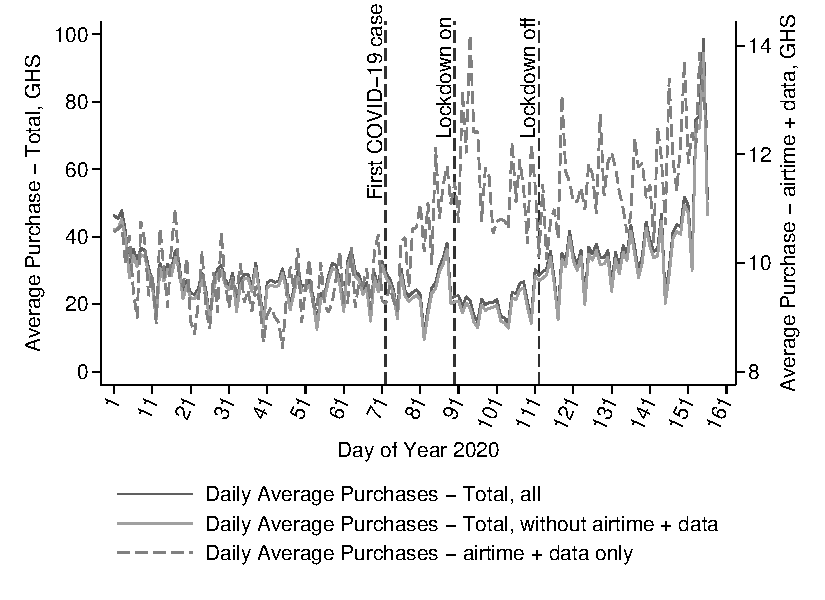
\includegraphics{../3-replication-package/original_figures/mobilefinTransactions}}{\large\par}
\par\end{centering}
\noindent Note: Mobile financial transaction data from a major local
telecommunications company and based on 694,695 transactions (2,0751
random unique subscribers). As displayed, average purchase (total
and total without airtime + data) shown in the left vertical axis
with solid lines, while average purchase for airtime-related activities
(airtime + data only) shown in the right vertical axis with a dash
line. Overall market activity decreased following the onset of the
pandemic, but demand for mobile airtime-related activities sharply
increased over the period. Pre-COVID-19, these two purchases (average
totals versus average airtime) look similar.
\end{figure}
}{\large\par}
\par\end{center}

\end{landscape}

\newpage{}

\subsection{Descriptive Statistics}
\begin{center}
{\large{}
\begin{table}[H]
{\large\caption{\textbf{S}{\footnotesize\textbf{UMMARY STATISTICS OF RELEVANT VARIABLES}}{\large\textbf{
}}{\footnotesize\textbf{\protect\label{tab:summary-baseSurvey-all}}}}
}{\large\par}

\begin{ThreePartTable}
\begin{table}[tbp]\centering
\def\sym#1{\ifmmode^{#1}\else\(^{#1}\)\fi}
\caption{Attrition}
\begin{tabular}{lccc}
\hline
Variable & Mean & SD & N \\
\hline\hline
\textbf{Demographic Characteristics} & & & \\ 
Female 0-1 & 0.147 & 0.354 & 1,130 \\ 
Akan ethnic 0-1 & 0.363 & 0.481 & 1,130 \\ 
Married 0-1 & 0.912 & 0.284 & 1,130 \\ 
Attained Junior High School (JHS) 0-1 & 0.783 & 0.412 & 1,130 \\ 
Household size (number) & 6.907 & 4.086 & 1,108 \\ 
Self-employed 0-1 & 0.764 & 0.425 & 1,130 \\ 
Operates in informal sector 0-1 & 0.801 & 0.400 & 1,130 \\ 
Personal income (1 to 5 scale) (monthly) & 1.621 & 0.898 & 1,106 \\ 
Staying together with mother 0-1 (Wave 0) & 0.067 & 0.251 & 1,130 \\ 
Has no religion 0-1 (Wave 0) & 0.054 & 0.226 & 1,130 \\ 
Staying together with spouse 0-1 (Wave 0) & 0.869 & 0.338 & 1,130 \\ 
Age at marriage (Years) (Wave 0) & 24.935 & 4.971 & 1,083 \\ 
\textbf{Poverty} & & & \\ 
Poverty rate (\%) (Schreiner 2005) (Wave 0) & 22.043 & 20.534 & 1,130 \\ 
\textbf{Pandemic Basics} & & & \\ 
Aware of COVID-19 0-1 & 0.996 & 0.060 & 1,106 \\ 
Trust Government's estimates about COVID-19 0-1 & 0.799 & 0.401 & 1,106 \\ 
In previously lockdown region 0-1 & 0.183 & 0.387 & 1,130 \\ 
Self does housework during pandemic 0-1 & 0.168 & 0.374 & 1,106 \\ 
Has relocated / moved in past 7 days 0-1 (Wave 2) & 0.014 & 0.119 & 977 \\ 
\textbf{Key Communication Constraints} & & & \\ 
Need to connect increased due to pandemic 0-1 & 0.701 & 0.458 & 1,105 \\ 
Unable to call in past 7 days 0-1 & 0.627 & 0.484 & 1,104 \\ 
Unable to call due to COVID-19 0-1 & 0.548 & 0.498 & 1,105 \\ 
Unable to make airtime transfers in past 7 days 0-1 & 0.474 & 0.500 & 1,104 \\ 
Borrow airtime 0-1 (Wave 2) & 0.319 & 0.466 & 977 \\ 
Seek digital loan 0-1 (Wave 2) & 0.088 & 0.283 & 977 \\ 
\textbf{Well-being Measures} & & & \\ 
Total Expenditure (GHS) (weekly) & 324.053 & 423.066 & 1,103 \\ 
Threatened Partner (1 = never to 4 = very often) & 1.194 & 0.700 & 1,103 \\ 
Hit Partner (1 = never to 4 = very often) & 1.194 & 0.700 & 1,103 \\ 
log K10 & 2.820 & 0.369 & 1,103 \\ 
Severe Distress 0-1 & 0.096 & 0.295 & 1,103 \\ 
I'm tired (mentally, emotionally, or socially) of COVID-19 0-1 & 0.538 & 0.499 & 1,105 \\ 
I'm depressed (1 = disagree to 5 = agree) & 1.599 & 0.942 & 1,103 \\ 
I'm relaxed (1 = disagree to 5 = agree) & 2.885 & 1.383 & 1,103 \\ 
I'm satisfied with life, all else equal (1 = disagree to 5 = agree) & 2.538 & 1.318 & 1,103 \\ 
I'm satisfied with finances, all else equal (1 = disagree to 5 = agree) & 2.075 & 1.157 & 1,103 \\ 
\hline\hline
\end{tabular}
\end{table}


\begin{spacing}{0.8}
Note: Observations are at the individual level. Table reports the
summary statistics of relevant variables from our baseline survey
waves. This include information about demographics, poverty indicators,
communication and well-being outcomes, respectively. The exchange
rate during the baseline period is US\$ 1.0 = GHS 5.80.
\end{spacing}
\end{table}
}{\large\par}
\par\end{center}

\begin{center}
{\large{}
\begin{figure}[H]
{\large\caption{\textbf{K}{\footnotesize\textbf{ 10 SCORE}}{\scriptsize\textbf{ AT
BASELINE (WAVE 1)\protect\label{fig:subjects_k10_base}}}}
}{\large\par}
\begin{centering}
{\large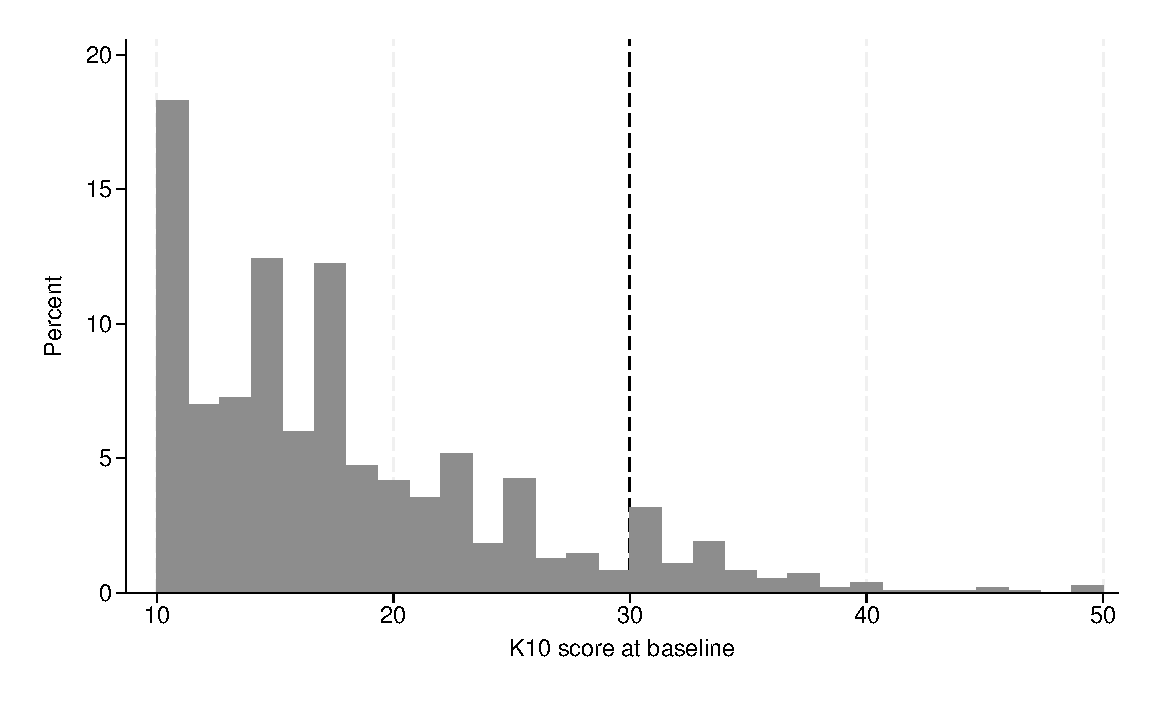
\includegraphics[scale=0.65]{../3-replication-package/Output/Figures/figure_a3}}{\large\par}
\par\end{centering}
Note: Observations are at the individual level. Low (scores of 10-15,
indicating little or no psychological distress). Moderate (scores
of 16-21). High (scores of 22-29). Very high or severe distress (scores
of 30-50). 11.5\% rate of severe distress (indicated by the vertical
dashed line).
\end{figure}
}{\large\par}
\par\end{center}

\begin{center}
{\large{}
\begin{figure}[H]
{\large\caption{\textbf{T}{\footnotesize\textbf{OTAL CONSUMPTION EXPENDITURE }}{\scriptsize\textbf{AT
BASELINE (WAVE 1)\protect\label{fig:subjects_totconsump_base}}}}
}{\large\par}
\begin{centering}
{\large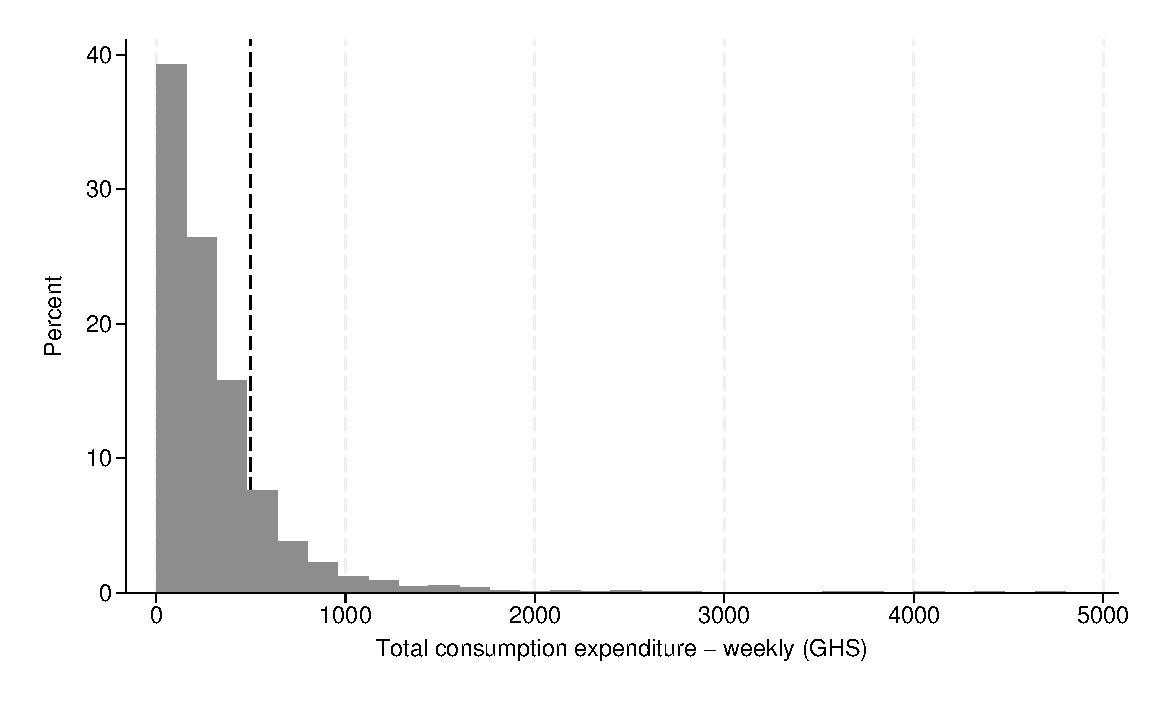
\includegraphics[scale=0.65]{../3-replication-package/Output/Figures/figure_a4}}{\large\par}
\par\end{centering}
Note: Observations are at the individual level. Total consumption
expenditure sums all expenses: food (inside and outside home), utilities,
personal care, education, health, and durables. 81.7\% rate of poor
consumption ($\leq$ 500GHS per week and indicated by the dashed vertical
line).
\end{figure}
}{\large\par}
\par\end{center}

\newpage{}

\subsection{Balance}
\begin{center}
{\large{}
\begin{table}[H]
{\large\caption{\textbf{B}{\footnotesize\textbf{ALANCE TEST: PRE-INTERVENTION TREATMENT-CONTROL
DIFFERENCES \protect\label{tab:treatment_balanceY}}}}
}{\large\par}

\include{../3-replication-package/Output/Tables/Table_a4}

\begin{spacing}{0.7}
Note: Observations are at the individual level. Each row is a separate
regression. Clustered standard errors (at the district level) are
reported in parentheses. {*}{*}{*} p<0.01, {*}{*} p<0.05, {*} p<0.10.
Mean baseline characteristics are also balanced across treatment arms.
\textbf{Results are similar with and without controls for randomization
strata dummies.}
\end{spacing}
\end{table}
}{\large\par}
\par\end{center}

\begin{center}
{\large{}
\begin{table}[H]
{\large\caption{\textbf{B}{\footnotesize\textbf{ALANCE TEST: PRE-INTERVENTION TREATMENT-CONTROL
DIFFERENCES \protect\label{tab:treatment_balanceXs}}}}
}{\large\par}

\include{../3-replication-package/Output/Tables/Table_a5}

\begin{spacing}{0.7}
Note: Observations are at the individual level. Each row is a separate
regression. The F and Chi-squared tests are conducted using the pooled
indicator \textbf{1(Communication Credit)} as the outcome and excluding
all the communication and well-being outcomes. Clustered standard
errors (at the district level) are reported in parentheses. {*}{*}{*}
p<0.01, {*}{*} p<0.05, {*} p<0.10. Mean baseline characteristics are
also balanced across treatment arms. \textbf{Results are similar with
and without controls for randomization strata dummies.}
\end{spacing}
\end{table}
}{\large\par}
\par\end{center}

\begin{center}
{\large{}
\begin{figure}[H]
{\large\caption{\textbf{P}{\footnotesize\textbf{HONE CALLS AND REACHABILITY OF INDIVIDUALS}}{\scriptsize\textbf{\protect\label{fig:subjects_reachability}}}}
}{\large\par}
\centering{}{\large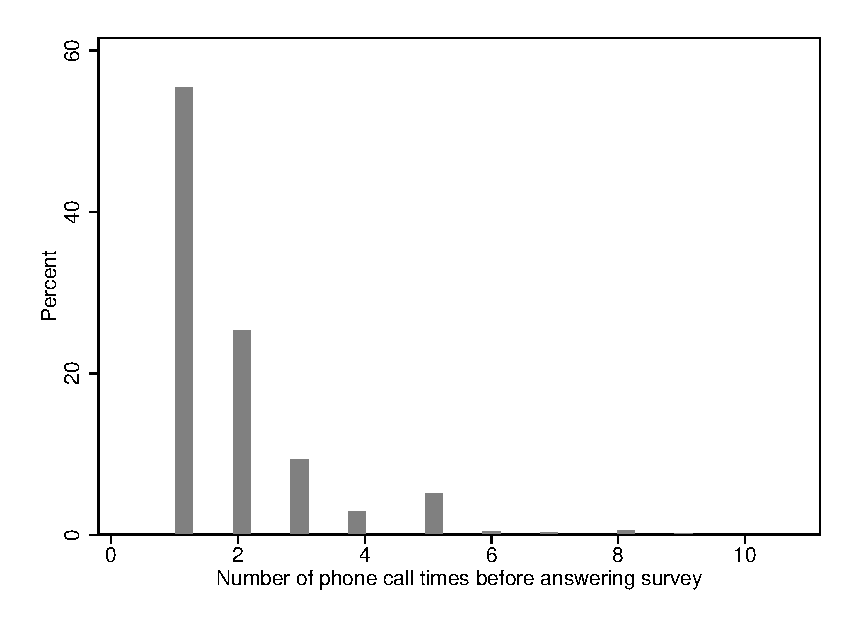
\includegraphics[scale=0.65]{../3-replication-package/Output/Figures/figure_a5}}{\large\par}
\end{figure}
}{\large\par}
\par\end{center}

\newpage{}
\begin{doublespace}

\subsection{Further Results \textendash{} Tables and Figures}
\end{doublespace}
\begin{center}
\textbf{POOLED EFFECTS OVER TRAJECTORY}
\par\end{center}

\begin{center}
{\large{}
\begin{figure}[H]
{\large\caption{{\footnotesize\textbf{MITIGATION OF COMMUNICATION CONSTRAINTS }}{\scriptsize\textbf{\protect\label{fig:mitigate_trajectory_meta}}}}
}{\large\par}
\begin{centering}
{\large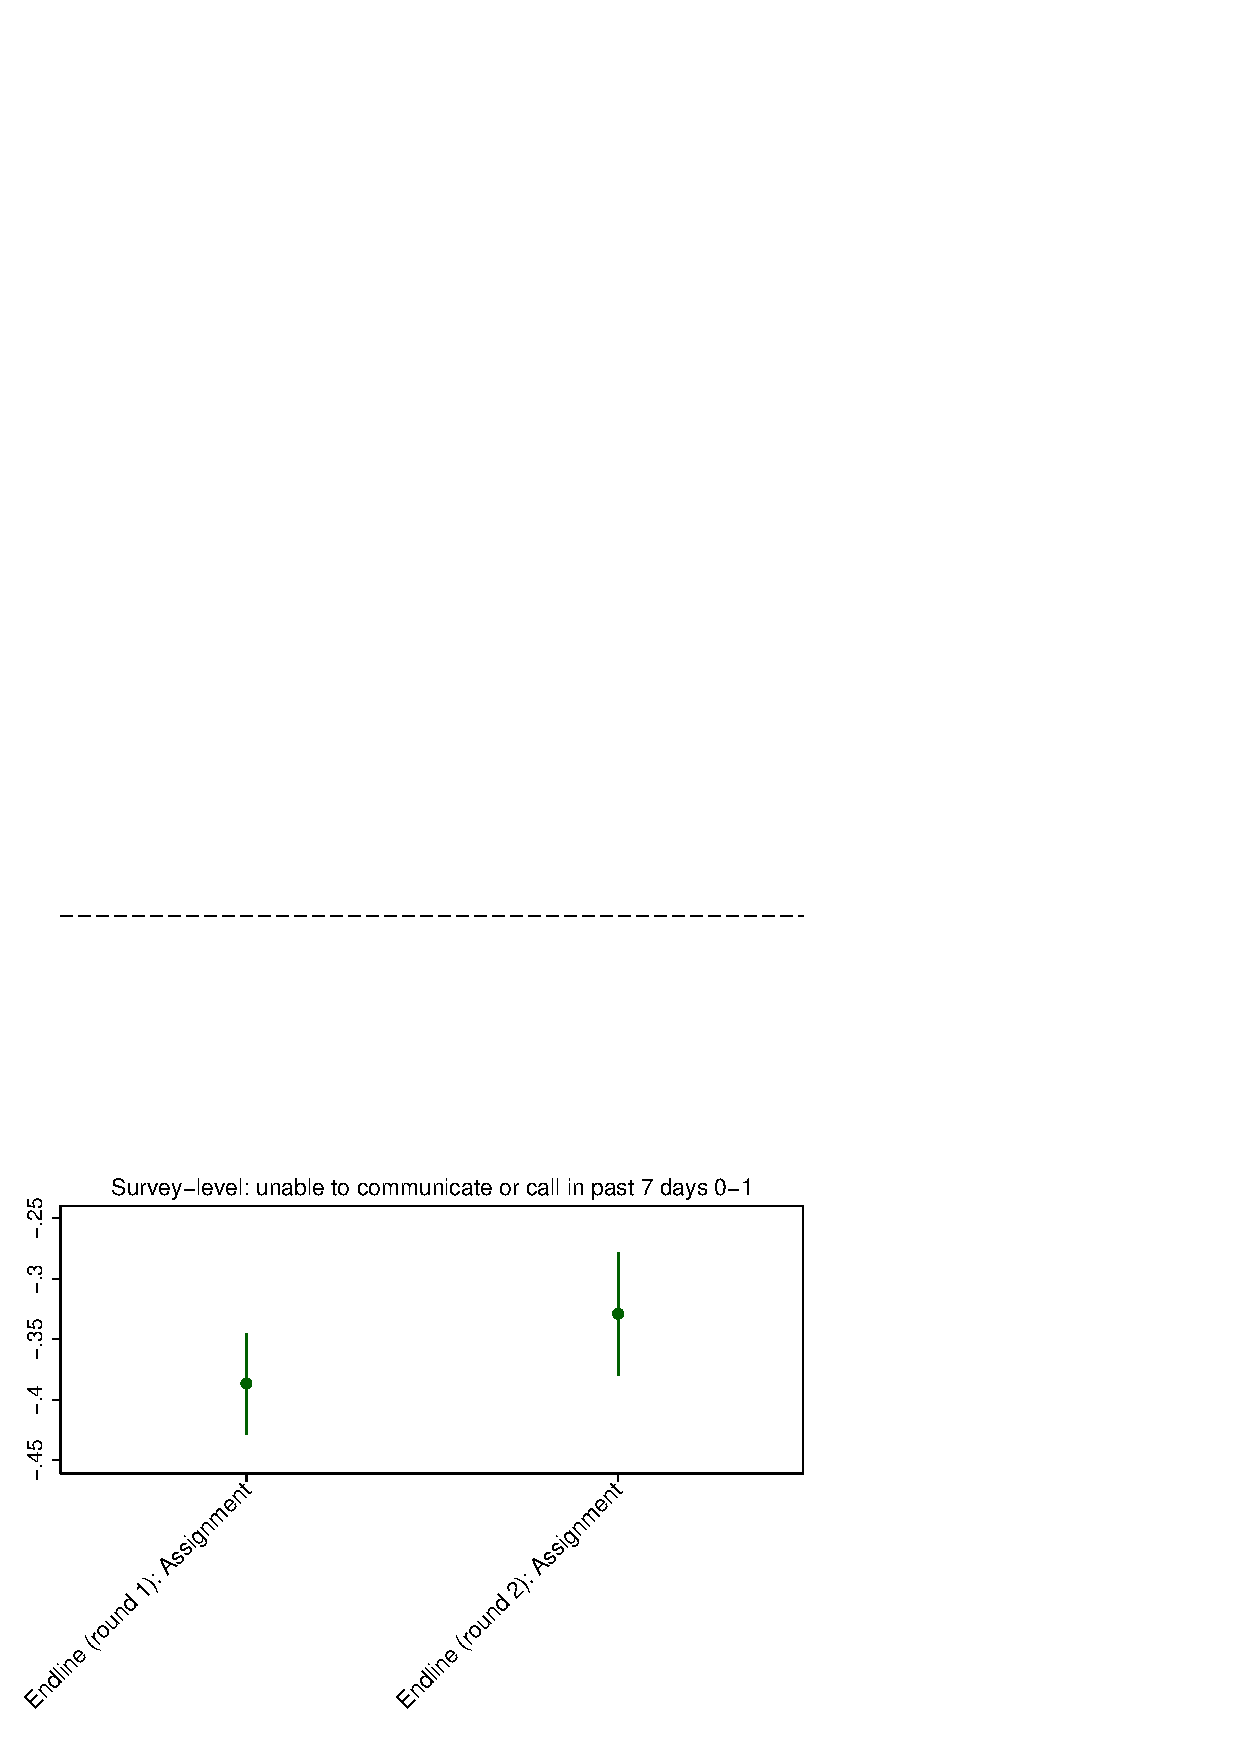
\includegraphics[scale=0.55]{../3-replication-package/Output/Figures/figure_a6_1}...\includegraphics[scale=0.55]{../3-replication-package/Output/Figures/figure_a6_2}}\\
{\large\par}
\par\end{centering}
\begin{centering}
{\large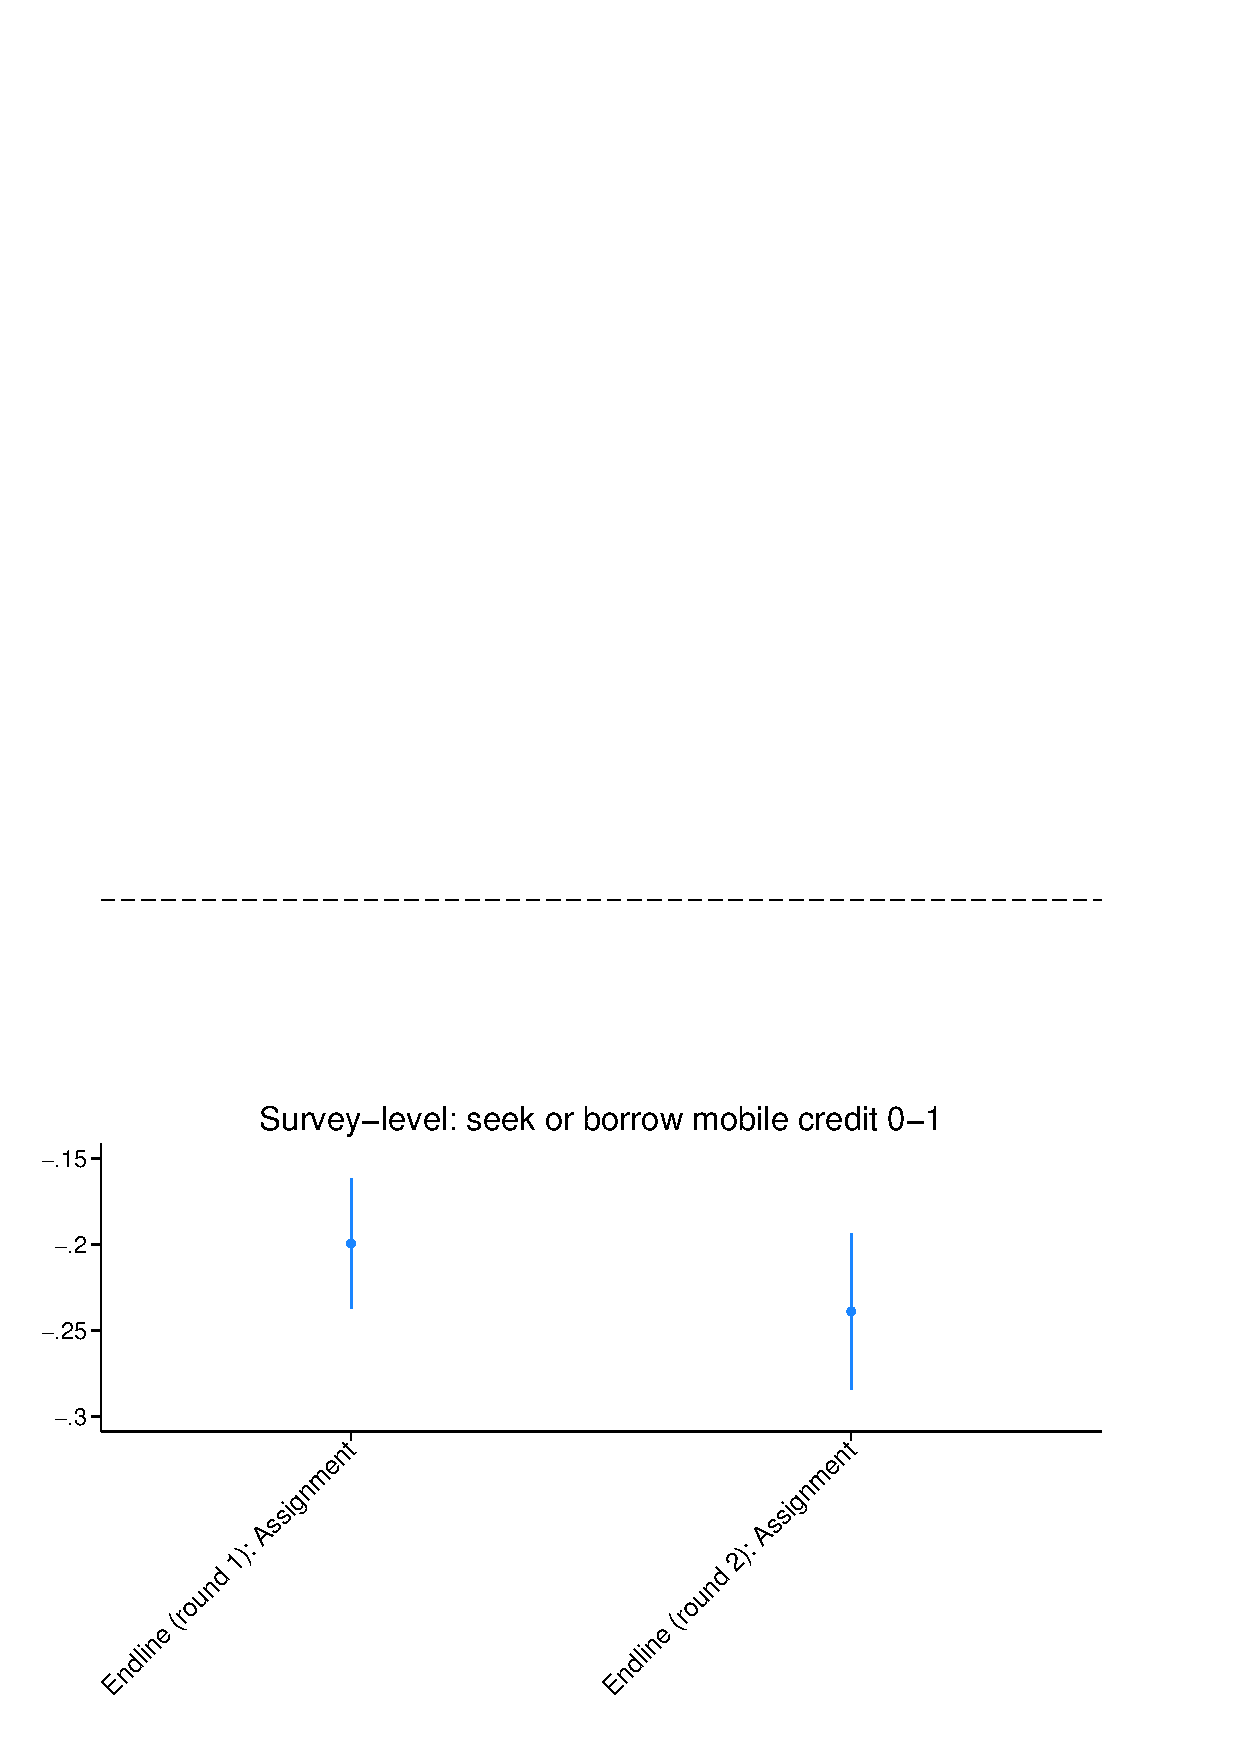
\includegraphics[scale=0.55]{../3-replication-package/Output/Figures/figure_a6_3}...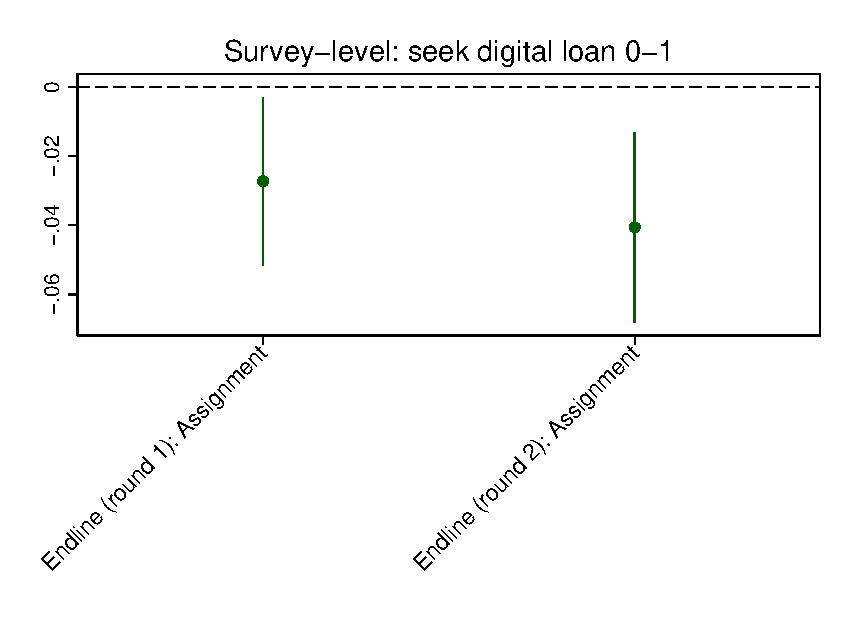
\includegraphics[scale=0.55]{../3-replication-package/Output/Figures/figure_a6_4}}{\large\par}
\par\end{centering}
{\large\vspace*{0.2cm}
}Note: Estimates are from a model that includes randomization strata
(district) fixed effects, survey date fixed effects, and double-post
LASSO specification which considers all individual controls, and individual
district and survey date fixed effects in the possible control set.
Controls include: individual\textquoteright s age, 0-1 indicator for
whether married or not, 0-1 indicator for whether belongs to akan
ethnic group or not, 0-1 indicator for whether self employed or not,
household size, 0-1 indicator for whether operates in the informal
sector, monthly personal income over an ordinal scale of 1 to 5, 0-1
indicator for whether attained junior high school (JHS) education,
and individual\textquoteright s gender. Observations are at the subject
$\times$ date level. Standard errors are clustered at the individual
level (the level of treatment). 90\% confidence intervals are displayed
around the estimates. Table of coefficients and standard errors available
upon request.
\end{figure}
}{\large\par}
\par\end{center}

\begin{center}
{\large{}
\begin{figure}[H]
{\large\caption{{\footnotesize\textbf{IMPACTS OF COMMUNICATION PROGRAMS ON WELL-BEING
MEASURES }}{\scriptsize\textbf{\protect\label{fig:consumpxhealth_trajectory_meta}}}}
}{\large\par}
\begin{centering}
{\large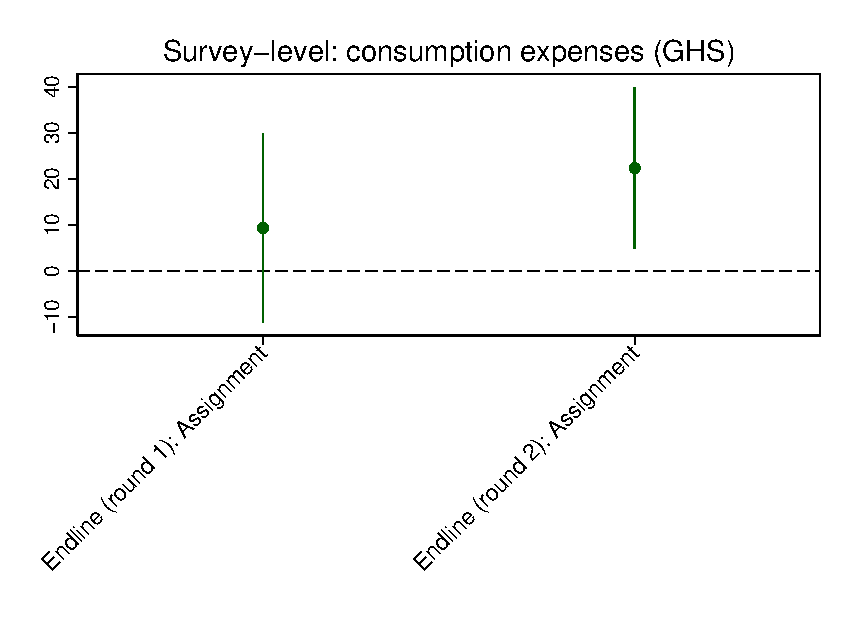
\includegraphics[scale=0.5]{../3-replication-package/Output/Figures/figure_a7_1}...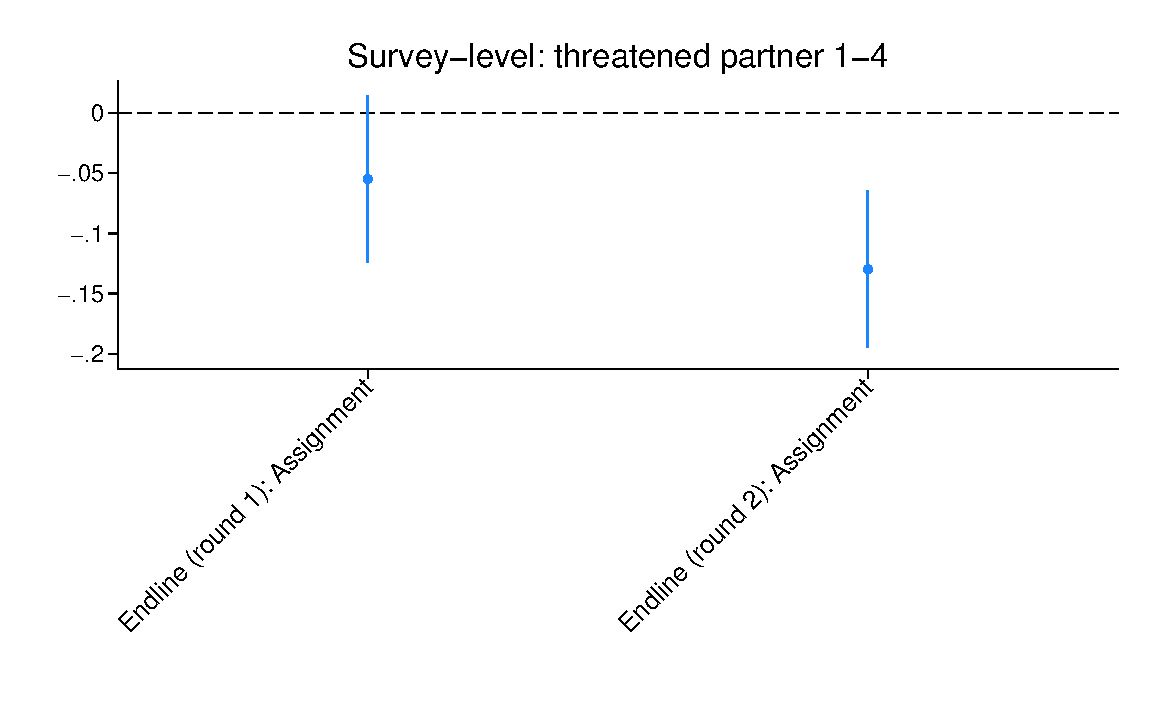
\includegraphics[scale=0.5]{../3-replication-package/Output/Figures/figure_a7_2}}{\small}\\
{\small\par}
\par\end{centering}
\begin{centering}
{\large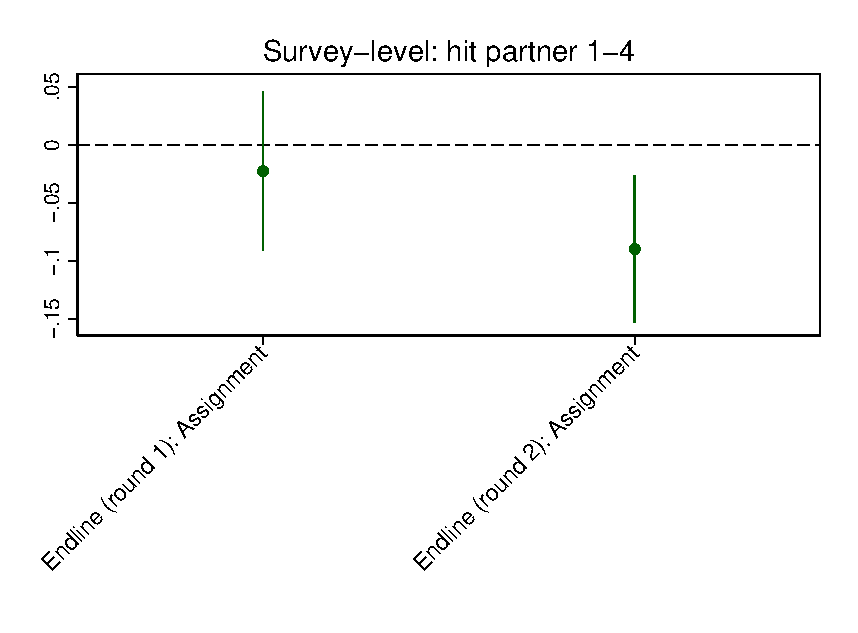
\includegraphics[scale=0.55]{../3-replication-package/Output/Figures/figure_a7_3}}\\
{\large\par}
\par\end{centering}
\begin{centering}
{\large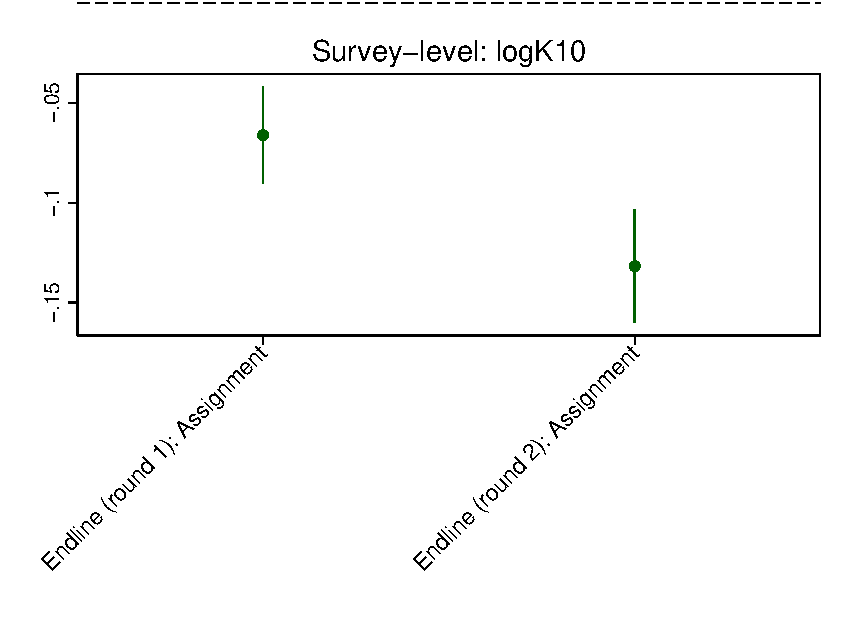
\includegraphics[scale=0.5]{../3-replication-package/Output/Figures/figure_a7_4}...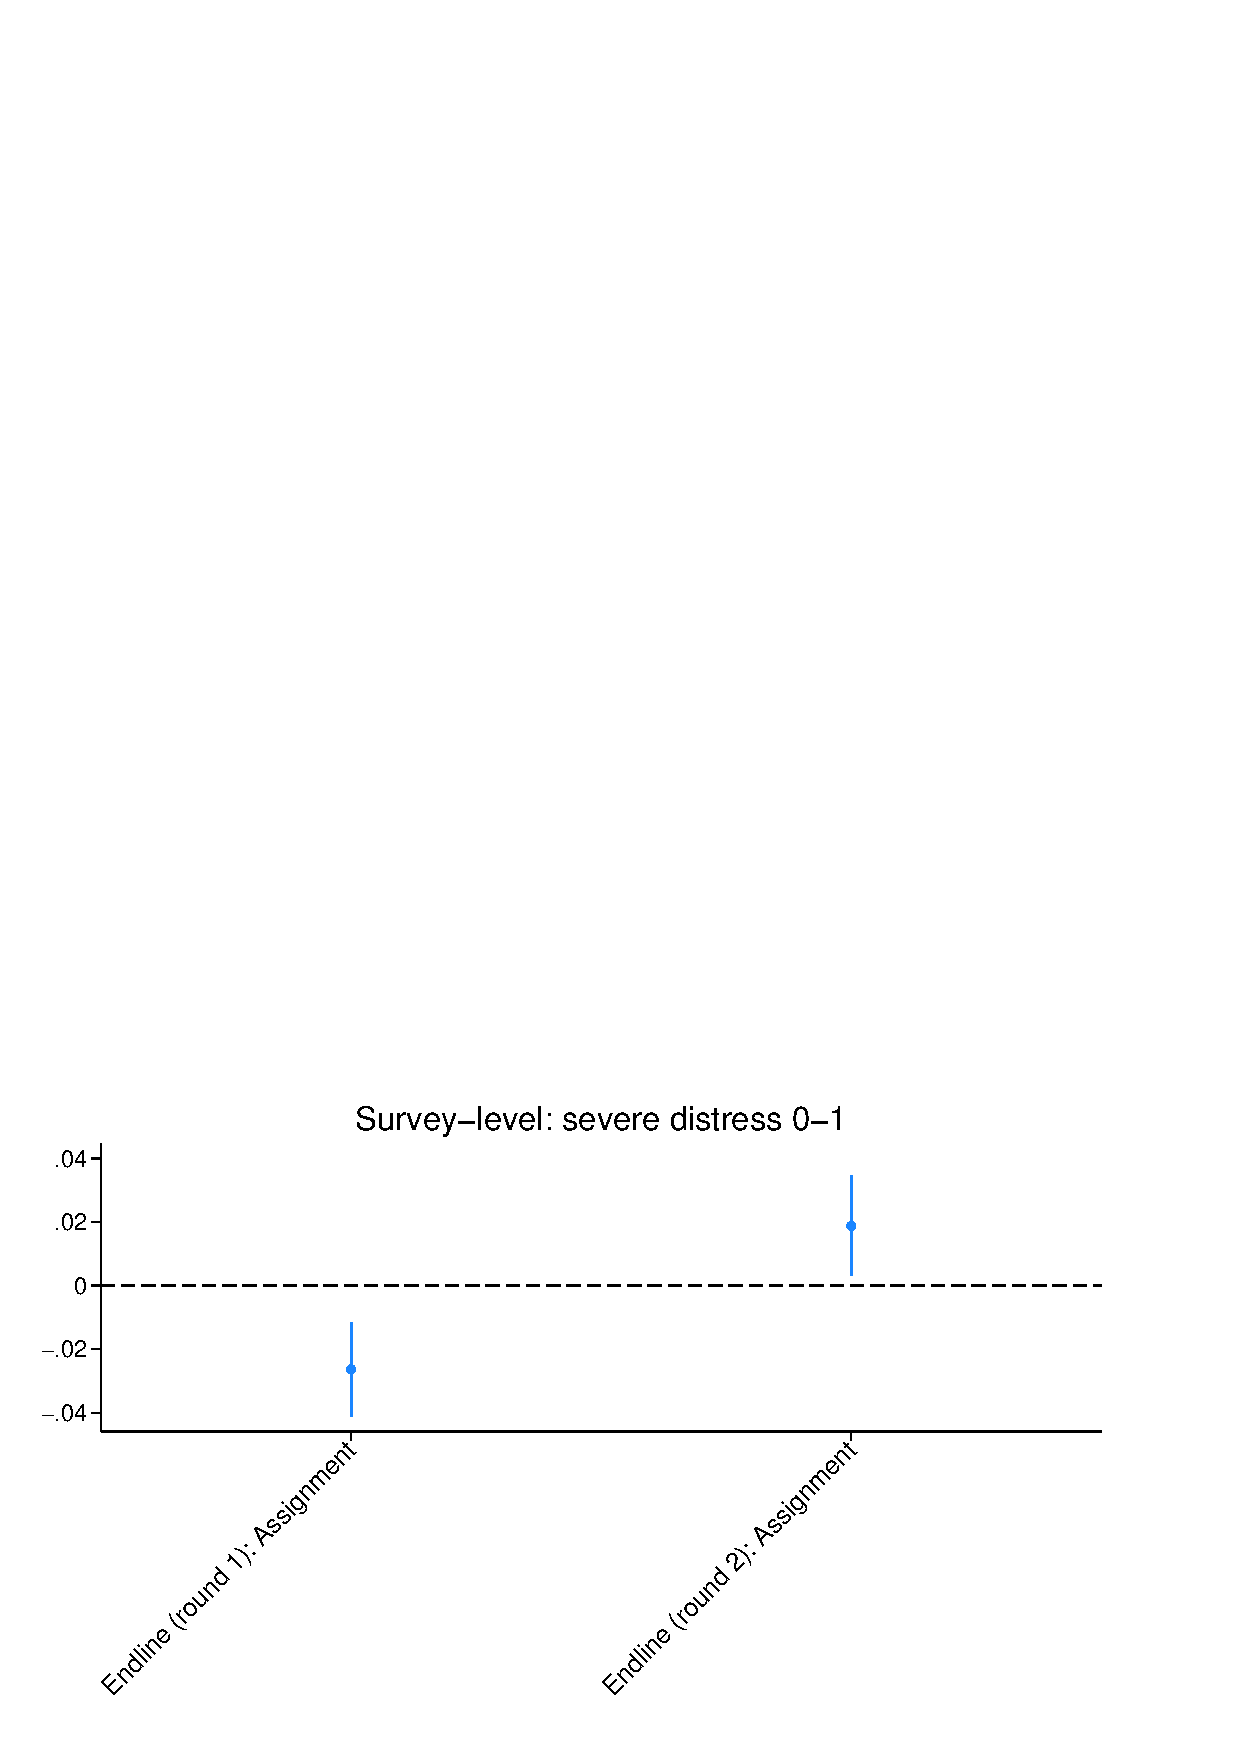
\includegraphics[scale=0.5]{../3-replication-package/Output/Figures/figure_a7_5}}{\large\par}
\par\end{centering}
{\large\vspace*{0.2cm}
}Note: Estimates are from a model that includes randomization strata
(district) fixed effects, survey date fixed effects, and double-post
LASSO specification which considers all individual controls, and individual
district and survey date fixed effects in the possible control set.
Controls include: individual\textquoteright s age, 0-1 indicator for
whether married or not, 0-1 indicator for whether belongs to akan
ethnic group or not, 0-1 indicator for whether self employed or not,
household size, 0-1 indicator for whether operates in the informal
sector, monthly personal income over an ordinal scale of 1 to 5, 0-1
indicator for whether attained junior high school (JHS) education,
and individual\textquoteright s gender. Observations are at the subject
$\times$ date level. Standard errors are clustered at the individual
level (the level of treatment). 90\% confidence intervals are displayed
around the estimates. Table of coefficients and standard errors available
upon request.
\end{figure}
}{\large\par}
\par\end{center}

\newpage{}
\begin{center}
\textbf{SEPARATE EFFECTS OVER TRAJECTORY}
\par\end{center}

\begin{center}
{\large{}
\begin{figure}[H]
{\large\caption{{\footnotesize\textbf{MITIGATION OF COMMUNICATION CONSTRAINTS }}{\scriptsize\textbf{\protect\label{fig:mitigate_trajectory_sep}}}}
}{\large\par}
\begin{centering}
{\large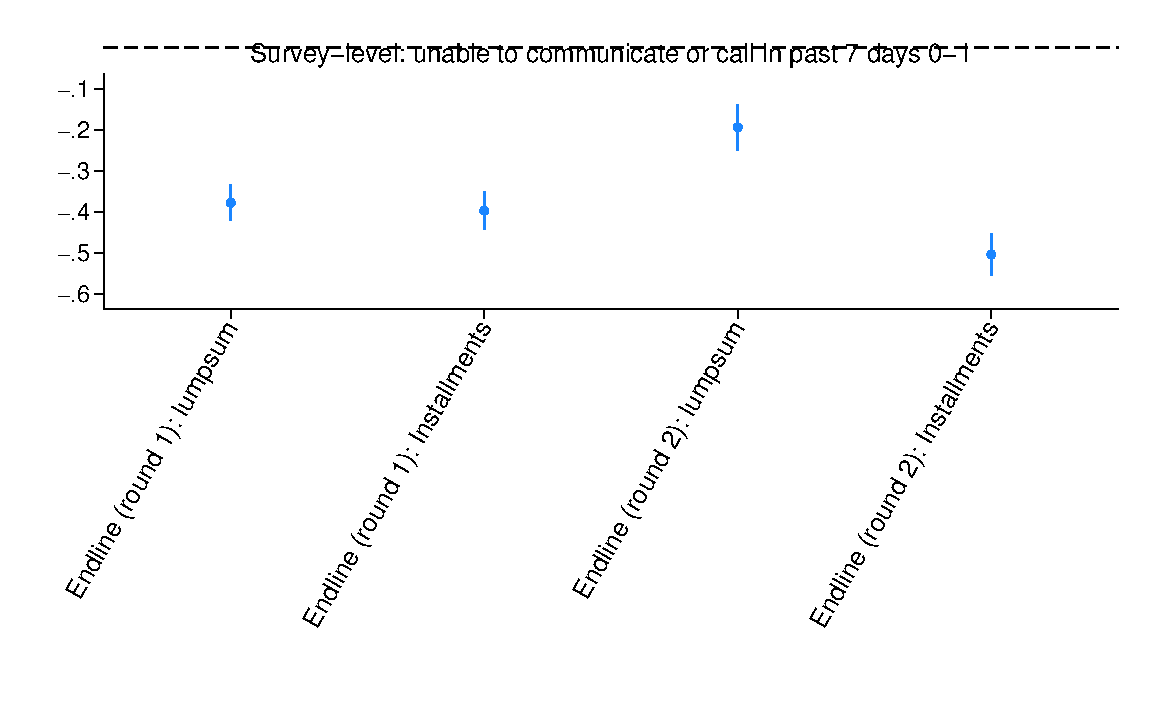
\includegraphics[scale=0.55]{../3-replication-package/Output/Figures/figure_a8_1}...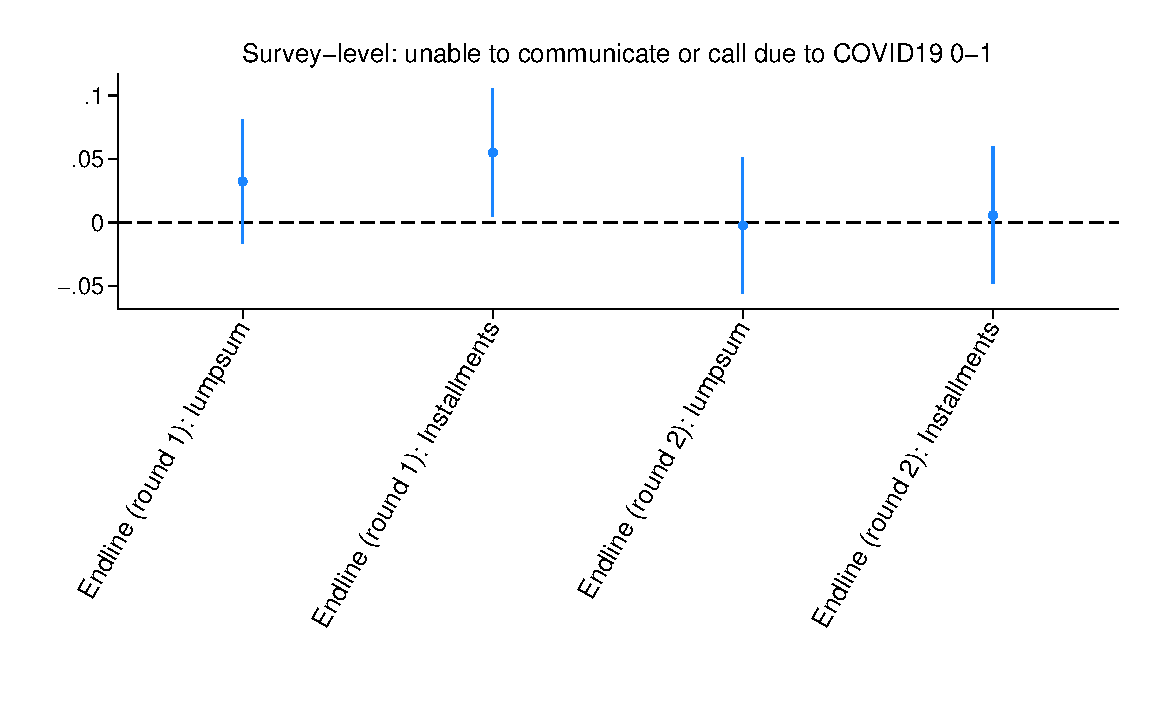
\includegraphics[scale=0.55]{../3-replication-package/Output/Figures/figure_a8_2}}\\
{\large\par}
\par\end{centering}
\begin{centering}
{\large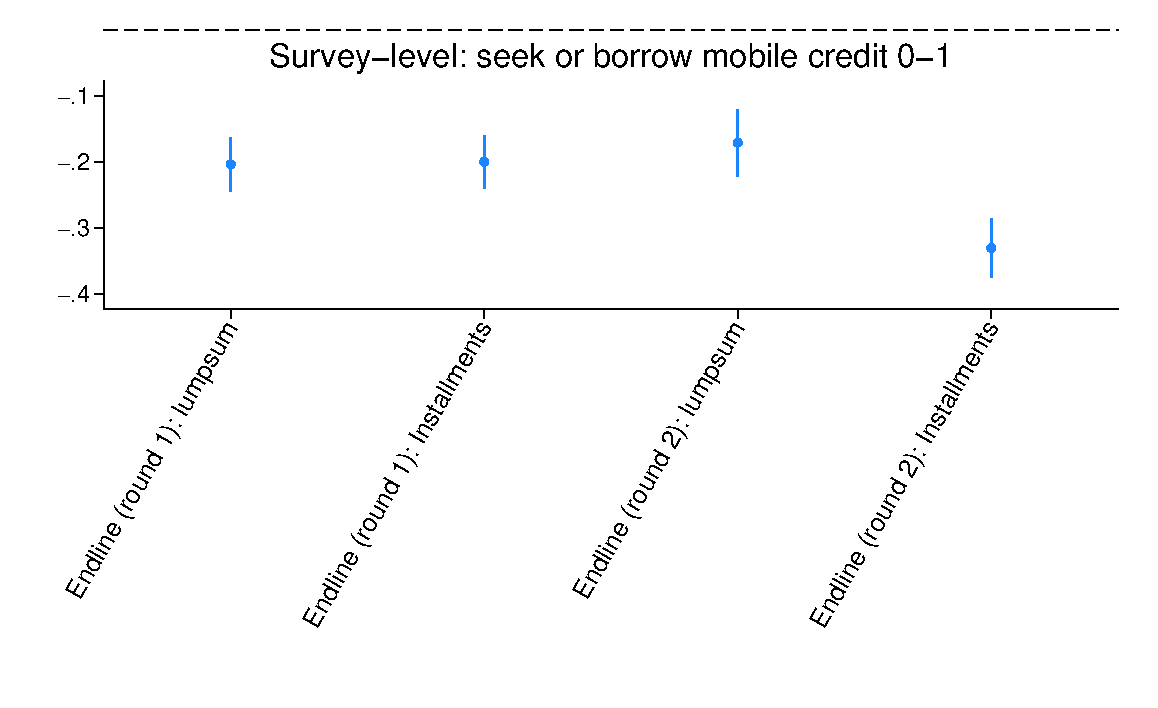
\includegraphics[scale=0.55]{../3-replication-package/Output/Figures/figure_a8_3}...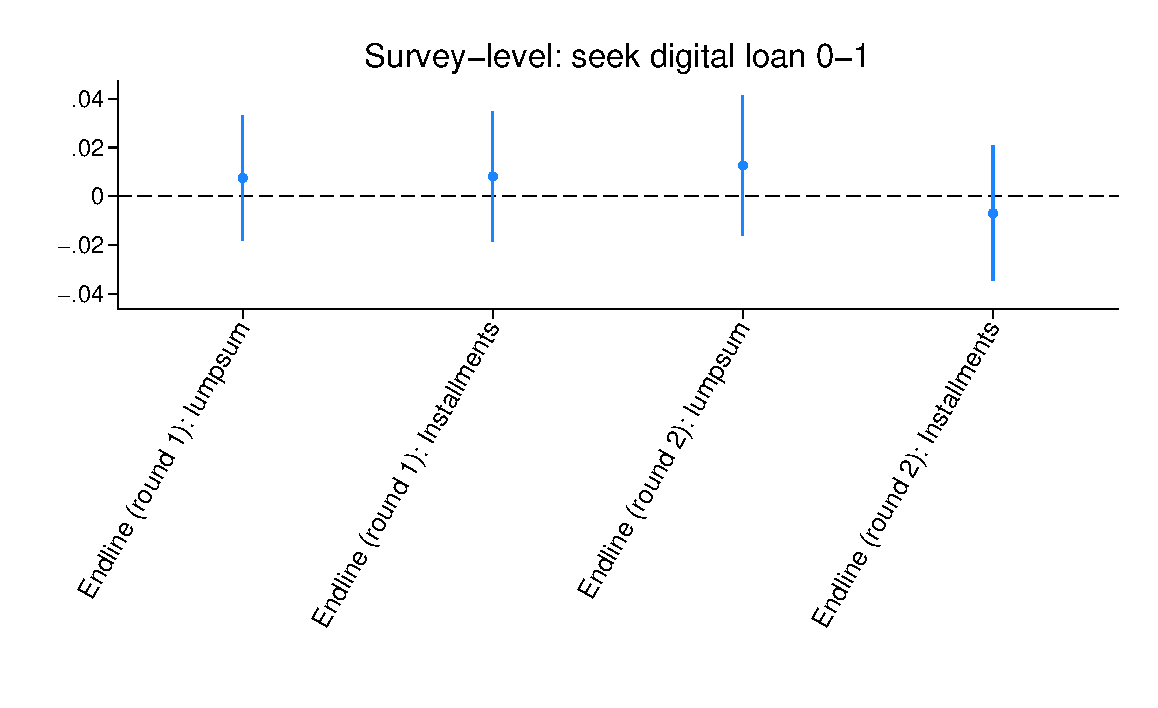
\includegraphics[scale=0.55]{../3-replication-package/Output/Figures/figure_a8_4}}{\large\par}
\par\end{centering}
{\large\vspace*{0.2cm}
}Note: Estimates are from a model that includes randomization strata
(district) fixed effects, survey date fixed effects, and double-post
LASSO specification which considers all individual controls, and individual
district and survey date fixed effects in the possible control set.
Controls include: individual\textquoteright s age, 0-1 indicator for
whether married or not, 0-1 indicator for whether belongs to akan
ethnic group or not, 0-1 indicator for whether self employed or not,
household size, 0-1 indicator for whether operates in the informal
sector, monthly personal income over an ordinal scale of 1 to 5, 0-1
indicator for whether attained junior high school (JHS) education,
and individual\textquoteright s gender. Observations are at the subject
$\times$ date level. Standard errors are clustered at the individual
level (the level of treatment). 90\% confidence intervals are displayed
around the estimates. Table of coefficients and standard errors available
upon request.
\end{figure}
}{\large\par}
\par\end{center}

\begin{center}
{\large{}
\begin{figure}[H]
{\large\caption{{\footnotesize\textbf{IMPACTS OF COMMUNICATION PROGRAMS ON WELL-BEING}}{\scriptsize\textbf{\protect\label{fig:consumpxhealth_trajectory_sep}}}}
}{\large\par}
\begin{centering}
{\large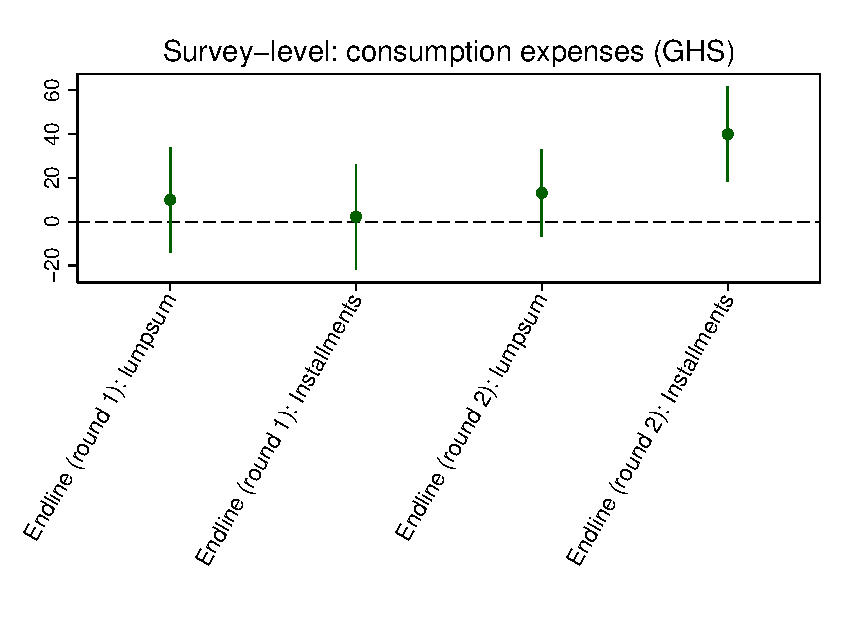
\includegraphics[scale=0.5]{../3-replication-package/Output/Figures/figure_a9_1}...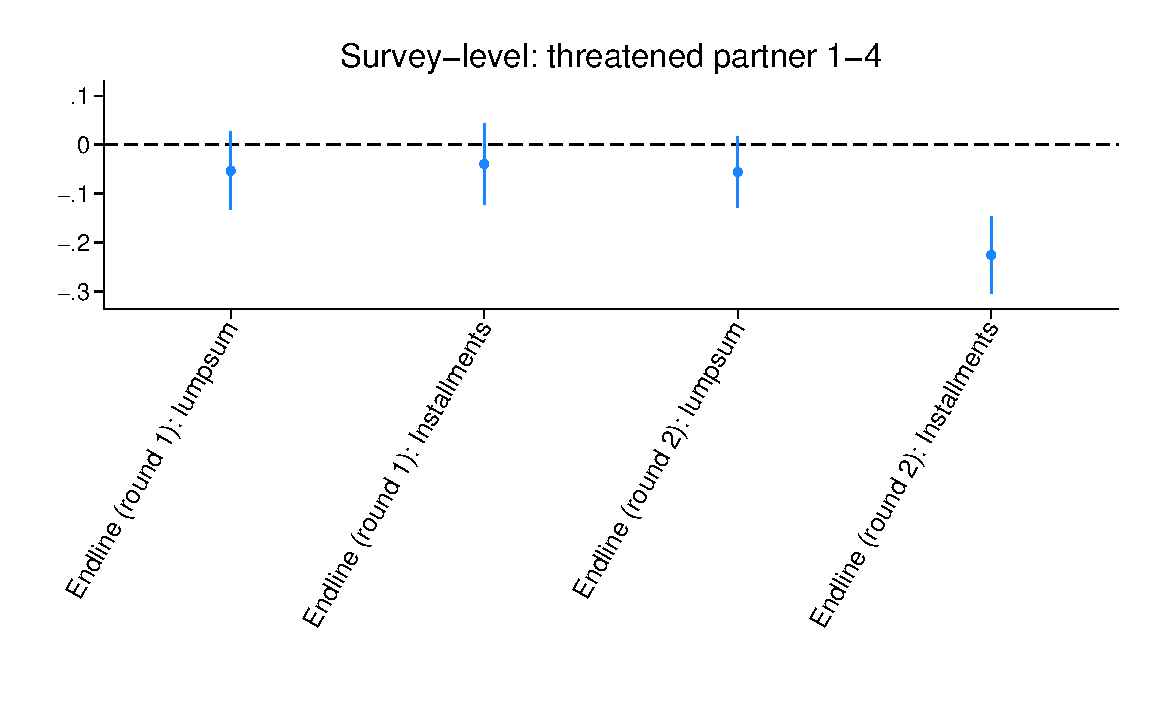
\includegraphics[scale=0.5]{../3-replication-package/Output/Figures/figure_a9_2}}{\small}\\
{\small\par}
\par\end{centering}
\begin{centering}
{\large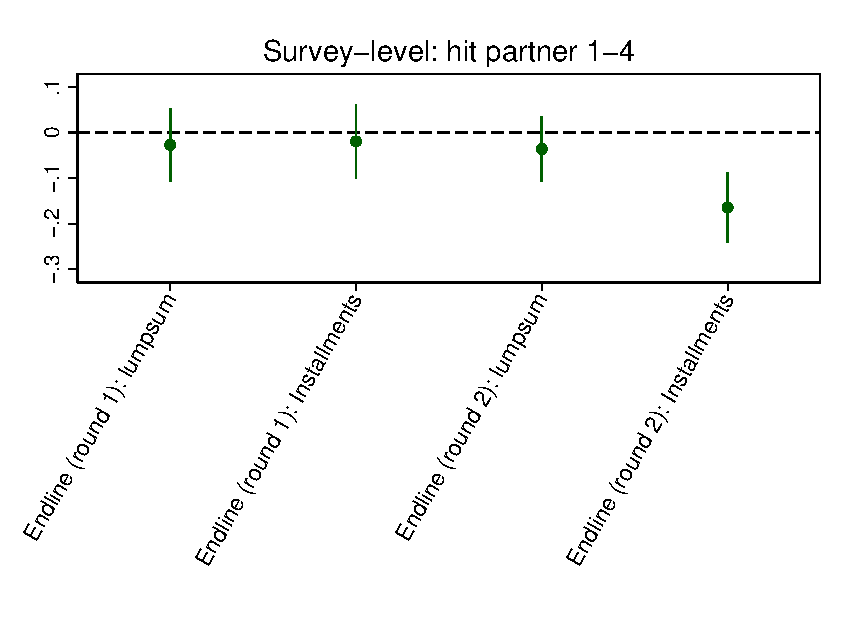
\includegraphics[scale=0.55]{../3-replication-package/Output/Figures/figure_a9_3}}\\
{\large\par}
\par\end{centering}
\begin{centering}
{\large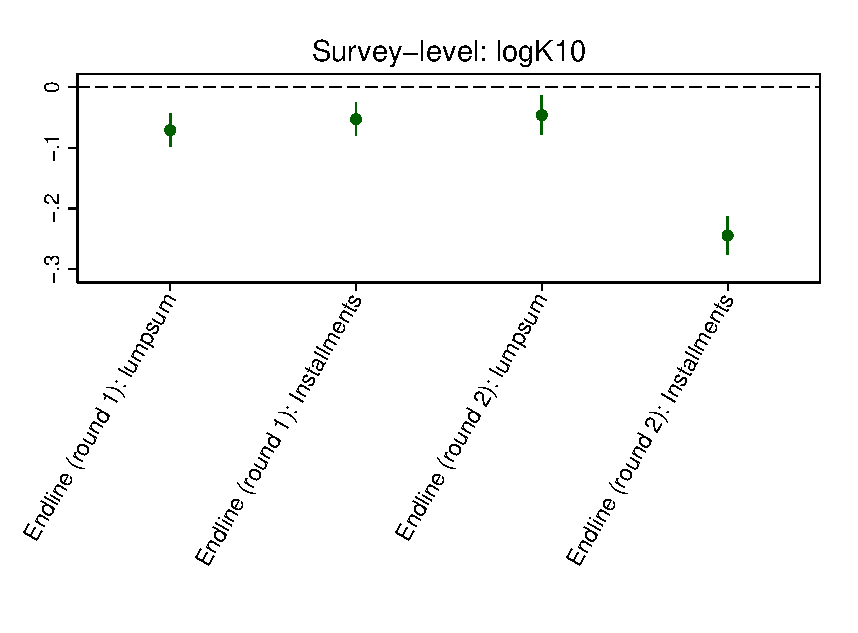
\includegraphics[scale=0.5]{../3-replication-package/Output/Figures/figure_a9_4}...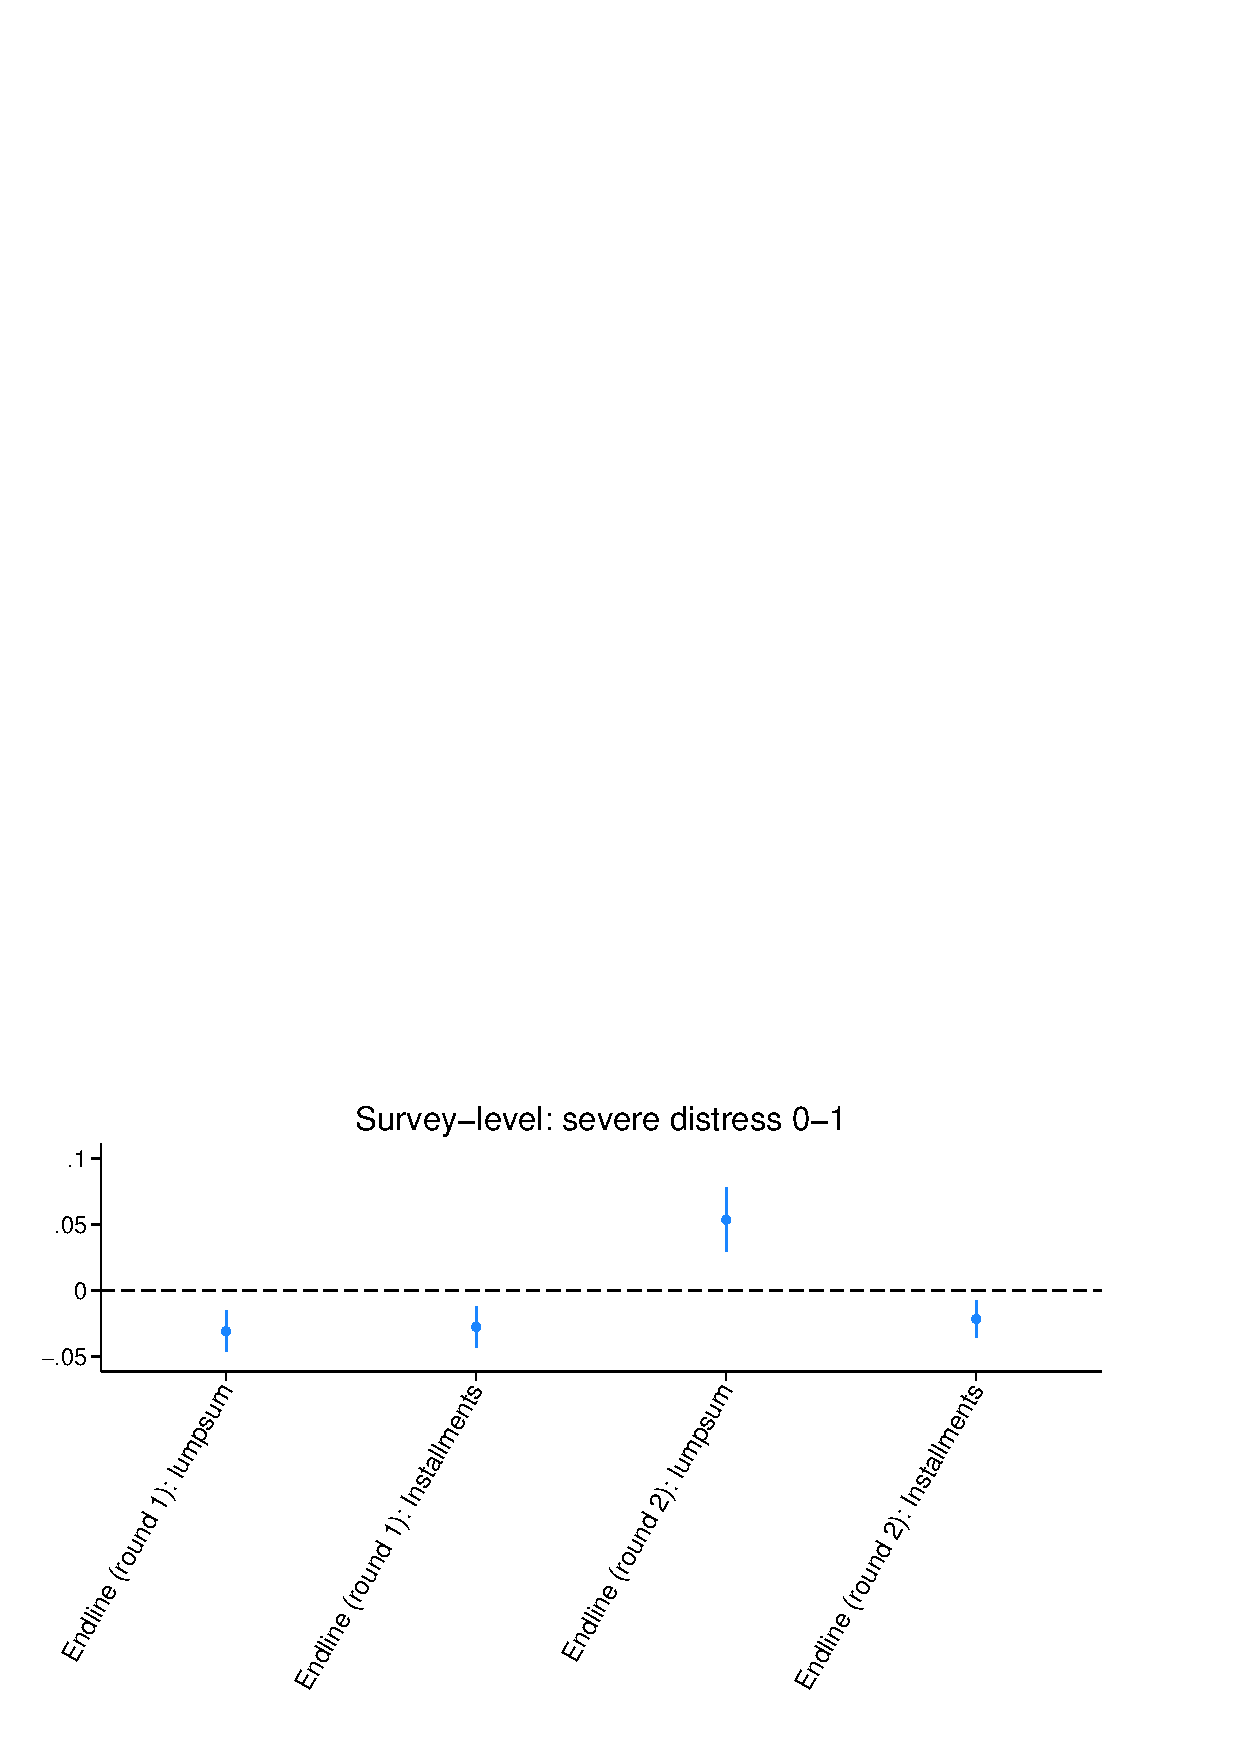
\includegraphics[scale=0.5]{../3-replication-package/Output/Figures/figure_a9_5}}{\large\par}
\par\end{centering}
{\large\vspace*{0.2cm}
}Note: Estimates are from a model that includes randomization strata
(district) fixed effects, survey date fixed effects, and double-post
LASSO specification which considers all individual controls, and individual
district and survey date fixed effects in the possible control set.
Controls include: individual\textquoteright s age, 0-1 indicator for
whether married or not, 0-1 indicator for whether belongs to akan
ethnic group or not, 0-1 indicator for whether self employed or not,
household size, 0-1 indicator for whether operates in the informal
sector, monthly personal income over an ordinal scale of 1 to 5, 0-1
indicator for whether attained junior high school (JHS) education,
and individual\textquoteright s gender. Observations are at the subject
$\times$ date level. Standard errors are clustered at the individual
level (the level of treatment). 90\% confidence intervals are displayed
around the estimates. Table of coefficients and standard errors available
upon request.
\end{figure}
}{\large\par}
\par\end{center}

\newpage{}

\noindent\begin{landscape}
\begin{center}
\textbf{HETEROGENEOUS EFFECTS}
\par\end{center}

\begin{center}
\begin{table}[!tph]
\caption{\textbf{I}{\footnotesize\textbf{MPACTS OF COMMUNICATION PROGRAMS ON
WELL-BEING BY POVERTY \protect\label{tab:wellbeingXpoverty_pooled_meta}}}}

\include{../3-replication-package/Output/Tables/Table_a6}

{\large\vspace*{0.2cm}
}Note: District is the randomization strata. The double-post LASSO
specification considers all individual controls, and individual district
and survey date fixed effects in the possible control set. Controls
include: individual\textquoteright s age, 0-1 indicator for whether
married or not, 0-1 indicator for whether belongs to akan ethnic group
or not, 0-1 indicator for whether self employed or not, household
size, 0-1 indicator for whether operates in the informal sector, monthly
personal income over an ordinal scale of 1 to 5, 0-1 indicator for
whether attained junior high school (JHS) education, and individual\textquoteright s
gender. Observations are at the subject $\times$ date level. Clustered
standard errors (at the individual level; the level of treatment)
are reported in parentheses. {*}{*}{*} p<0.01 (1\% level), {*}{*}
p<0.05 (5\% level), {*} p<0.1 (10\% level). Romano-Wolf multiple hypothesis
correction \textit{p}-values (Romano and Wolf {[}2005{]}) reported
separately for consumption expense outcomes family (Total (GHS) Expenditure;
Food-In (GHS); Food-Out (GHS); Utilities (GHS); Personal care (GHS);
Educ. (GHS); Health (GHS); Durables (GHS)), and for mental health
and domestic violence outcomes family (Threatened Partner 1-4; Hit
Partner 1-4; log K10; Severe Distress 0-1). NE denotes not estimable.
\end{table}
\par\end{center}

\begin{center}
\begin{table}[!tph]
\caption{\textbf{I}{\footnotesize\textbf{MPACTS OF COMMUNICATION PROGRAMS ON
WELL-BEING BY INFORMALITY \protect\label{tab:wellbeingXinformal_pooled_meta}}}}

\include{../3-replication-package/Output/Tables/Table_a7}

{\large\vspace*{0.2cm}
}Note: District is the randomization strata. The double-post LASSO
specification considers all individual controls, and individual district
and survey date fixed effects in the possible control set. Controls
include: individual\textquoteright s age, 0-1 indicator for whether
married or not, 0-1 indicator for whether belongs to akan ethnic group
or not, 0-1 indicator for whether self employed or not, household
size, 0-1 indicator for whether operates in the informal sector, monthly
personal income over an ordinal scale of 1 to 5, 0-1 indicator for
whether attained junior high school (JHS) education, and individual\textquoteright s
gender. Observations are at the subject $\times$ date level. Clustered
standard errors (at the individual level; the level of treatment)
are reported in parentheses. {*}{*}{*} p<0.01 (1\% level), {*}{*}
p<0.05 (5\% level), {*} p<0.1 (10\% level). NE denotes not estimable,
which occurs due to insufficient sample from individuals in the informal
sector with severe mental distress experiences. Romano-Wolf multiple
hypothesis correction \textit{p}-values (Romano and Wolf {[}2005{]})
reported separately for consumption expense outcomes family (Total
(GHS) Expenditure; Food-In (GHS); Food-Out (GHS); Utilities (GHS);
Personal care (GHS); Educ. (GHS); Health (GHS); Durables (GHS)), and
for mental health and domestic violence outcomes family (Threatened
Partner 1-4; Hit Partner 1-4; log K10; Severe Distress 0-1).
\end{table}
\par\end{center}

\begin{center}
\begin{table}[!tph]
\caption{\textbf{I}{\footnotesize\textbf{MPACTS OF COMMUNICATION PROGRAMS ON
WELL-BEING BY GENDER \protect\label{tab:wellbeingXfemale_pooled_meta}}}}

\include{../3-replication-package/Output/Tables/Table_a8}

{\large\vspace*{0.2cm}
}Note: District is the randomization strata. The double-post LASSO
specification considers all individual controls, and individual district
and survey date fixed effects in the possible control set. Controls
include: individual\textquoteright s age, 0-1 indicator for whether
married or not, 0-1 indicator for whether belongs to akan ethnic group
or not, 0-1 indicator for whether self employed or not, household
size, 0-1 indicator for whether operates in the informal sector, monthly
personal income over an ordinal scale of 1 to 5, 0-1 indicator for
whether attained junior high school (JHS) education, and individual\textquoteright s
gender. Observations are at the subject $\times$ date level. Clustered
standard errors (at the individual level; the level of treatment)
are reported in parentheses. {*}{*}{*} p<0.01 (1\% level), {*}{*}
p<0.05 (5\% level), {*} p<0.1 (10\% level). Romano-Wolf multiple hypothesis
correction \textit{p}-values (Romano and Wolf {[}2005{]}) reported
separately for consumption expense outcomes family (Total (GHS) Expenditure;
Food-In (GHS); Food-Out (GHS); Utilities (GHS); Personal care (GHS);
Educ. (GHS); Health (GHS); Durables (GHS)), and for mental health
and domestic violence outcomes family (Threatened Partner 1-4; Hit
Partner 1-4; log K10; Severe Distress 0-1).
\end{table}
\par\end{center}

\begin{center}
\begin{table}[!tph]
\caption{\textbf{I}{\footnotesize\textbf{MPACTS OF COMMUNICATION PROGRAMS ON
WELL-BEING BY LOCKED-DOWN \protect\label{tab:wellbeingXlockeddown_pooled_meta}}}}

\include{../3-replication-package/Output/Tables/Table_a9}

{\large\vspace*{0.2cm}
}Note: District is the randomization strata. The double-post LASSO
specification considers all individual controls, and individual district
and survey date fixed effects in the possible control set. Controls
include: individual\textquoteright s age, 0-1 indicator for whether
married or not, 0-1 indicator for whether belongs to akan ethnic group
or not, 0-1 indicator for whether self employed or not, household
size, 0-1 indicator for whether operates in the informal sector, monthly
personal income over an ordinal scale of 1 to 5, 0-1 indicator for
whether attained junior high school (JHS) education, and individual\textquoteright s
gender. Observations are at the subject $\times$ date level. Clustered
standard errors (at the individual level; the level of treatment)
are reported in parentheses. {*}{*}{*} p<0.01 (1\% level), {*}{*}
p<0.05 (5\% level), {*} p<0.1 (10\% level). Romano-Wolf multiple hypothesis
correction \textit{p}-values (Romano and Wolf {[}2005{]}) reported
separately for consumption expense outcomes family (Total (GHS) Expenditure;
Food-In (GHS); Food-Out (GHS); Utilities (GHS); Personal care (GHS);
Educ. (GHS); Health (GHS); Durables (GHS)), and for mental health
and domestic violence outcomes family (Threatened Partner 1-4; Hit
Partner 1-4; log K10; Severe Distress 0-1). NE denotes not estimable.
\end{table}
\par\end{center}

\noindent\end{landscape}
\begin{center}
{\large{}
\begin{figure}[H]
{\large\caption{\textbf{D}{\footnotesize\textbf{ISTRIBUTION OF CONSUMPTION GROWTH
AMONG INDIVIDUALS INSIDE AND OUTSIDE PANDEMIC'S LOCKDOWN AREAS}}{\tiny\textbf{
\protect\label{fig:_consumpShock?}}}}
}{\large\par}
\begin{centering}
{\large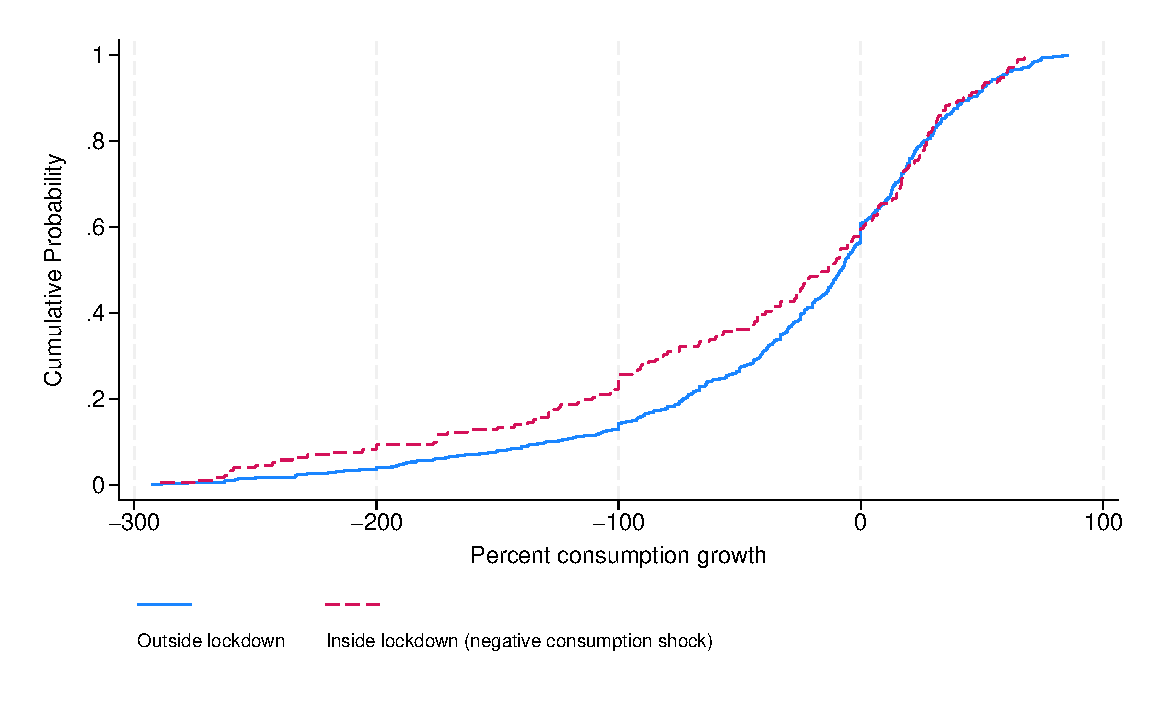
\includegraphics[scale=1.2]{../3-replication-package/Output/Figures/figure_a10}}{\large\par}
\par\end{centering}
{\small Note: Figure plots the distribution (CDF) of consumption growth
per week at endline for the different subsamples (lockdown areas vs
non-lockdown areas). Observations are at the individual level. Median
(mean) percent consumption growth is -13\% (-45\%) for individuals
in lockdown areas and -8\% (-27\%) for those in non-lockdown areas.
From a Kolmogorov\textendash Smirnov (KS) test for the equality of
distributions, }{\small\textit{p}}{\small -value equals 0.020 (for
equality test, we trimmed the individual consumption growth outcome
at the 5\% level). Equality tests reject the null that the distributional
pairs are equal.}{\small\par}
\end{figure}
}{\large\par}
\par\end{center}

\newpage{}

\subsection{Definition of Relevant Select Variables \textendash{} Questions}

\begin{doublespace}
\noindent{\large\textbf{Communication constraints (un)mitigation: }}{\large\par}
\end{doublespace}

\noindent{\large Consider the last 7 days: }{\large\par}
\begin{enumerate}
\item {\large Unable to call in past 7days 0-1: }{\large\texttt{Were you
confronted with the need to call others (i.e., family, friends or
work) but unable to call because you/ household lacked enough communication
resources to cover costs? 0=No, 1=Yes}}{\large\par}
\item {\large Borrow airtime 0-1: }{\large\texttt{Have borrowed airtime due
to unexpected circumstances to make calls? 0=No, 1=Yes }}{\large\par}
\item {\large Seek digital loan 0-1: }{\large\texttt{Have taken a digital
loan due to unexpected circumstances to make calls? 0=No, 1=Yes}}{\large\par}
\item {\large Unable to call due to COVID19 0-1: }{\large\texttt{Are you
sometimes unable to see or communicate with your family and friends
due to COVID19, its lockdown restrictions and other personal avoidance
steps you have taken? 0=No, 1=Yes }}{\large\par}
\end{enumerate}
\begin{doublespace}
\noindent{\large\textbf{Gender and Domestic violence relations: }}{\large\par}
\end{doublespace}

\noindent{\large Consider last 7 days: Please indicate how often you
act to the following:}\textbf{ }

\noindent\textbf{USE CODES:}

\noindent{\large\texttt{1=Never (less than 1 time in 7 days), 2=Sometime
(1-2 times in 7 days), 3=Often (3-4 times in 7 days), 4=Very often
(5-7 times in 7 days), 5=No Answer (if you want/feel uncomfortable
to say)}}{\large\par}
\begin{enumerate}
\item {\large Threatened Partner 1-4:}{\large\texttt{ How often do you threaten
to hurt your partner or someone close to your partner? }}{\large\par}
\item {\large Hit Partner 1-4:}{\large\texttt{ How often do you hit or throw
something at your partner? }}{\large\par}
\end{enumerate}
\begin{doublespace}
\noindent{\large\textbf{Mental Health (K10):}}{\large\par}
\end{doublespace}

\noindent{\large Consider last 7 days: Please indicate how often you
feel about the following: }{\large\par}

\noindent\textbf{USE CODES:}

\noindent{\large\texttt{1=None of the time (less than 1 time in 7
days), 2=A little of the time (1-2 times in 7 days), 3=Some of the
time (3-4 times in 7 days) 4=Most of the time (5-6 times in 7 days),
5=All of the time (7 times in 7 days) }}{\large\par}
\begin{enumerate}
\item {\large\texttt{About how often did you feel tired out for no good
reason? }}{\large\par}
\item {\large\texttt{About how often did you feel nervous? }}{\large\par}
\item {\large\texttt{About how often did you feel nervous that nothing could
calm you down? }}{\large\par}
\item {\large\texttt{About how often did you feel hopeless? }}{\large\par}
\item {\large\texttt{About how often did you feel restless or fidgety? }}{\large\par}
\item {\large\texttt{About how often did you feel so restless you could
not sit still? }}{\large\par}
\item {\large\texttt{About how often did you feel depressed? }}{\large\par}
\item {\large\texttt{About how often did you feel that everything was an
effort? }}{\large\par}
\item {\large\texttt{About how often did you feel so sad that nothing could
cheer you up? }}{\large\par}
\item {\large\texttt{About how often did you feel worthless?}}{\large\par}
\end{enumerate}
\noindent{\large\textbf{Consumption Expenditures (weekly):}}{\large\par}
\begin{enumerate}
\item {\large\texttt{What is the total value (in GHS) of all food and beverage
items your household (i) purchased and consumed, (ii) consumed from
your own stock or production, or (iii) received as a gift and consumed
over the last 7 days? NOTE: Please only include food and beverage
items consumed in the 7 days ...GHS }}{\large\par}
\item {\large\texttt{What is the total value (in GHS) of all food and beverage
items you or any member of your household purchased and consumed from
outside the house over the last 7 days? NOTE: This includes items
purchased outside the house in restaurants, cafeterias, canteens/kiosks,
as well as products such as spirits, tobacco, stimulants, etc. ...GHS}}{\large\par}
\item {\large\texttt{What is the total value (in GHS) of house rents, house
repair costs and utilities that were paid for, purchased, or acquired
from other sources (ie gifts and in-kind) by your household over the
last 7 days? NOTE: Utilities include sewerage, electricity, water,
gas, cooking fuels, house servants, etc. ...GHS }}{\large\par}
\item {\large\texttt{What is the total value (in GHS) of products and services
for personal use and care, that were paid for, purchased, or acquired
from other sources (ie gifts and in-kind) over the last 7 days by
your household? NOTE: Personal care products and services include
barber services, electrical appliances for personal care, oils, soaps,
etc. Personal use products and services include jewelry, accessories
(watches, clocks, clothing, etc.), cultural services, mobile airtime
services, financial service fees, transportation costs. ...GHS }}{\large\par}
\item {\large\texttt{What is the total value (in GHS) of education expenses
(i.e., all tuition or fees including all educational scholarships)
over the last 7 days by your household? ...GHS }}{\large\par}
\item {\large\texttt{What is the total value (in GHS) of consultation or
treatment services, and pharmaceutical or therapeutic products purchased
last 7 days by your household? ...GHS }}{\large\par}
\item {\large\texttt{What is the total value (in GHS) of durable products
such as furniture, electronics and other household appliances, purchased
over the last 7 days by your household? NOTE: This includes furniture,
household appliances (large and small), repair of household appliances,
miscellaneous accessories such as TVs, laptops, cars, mobile phones,
bicycles, torches, batteries, solar lamps, etc. ...GHS }}{\large\par}
\item {\large\texttt{Total expenditure: add 1 to 8 ...GHS}}
%
\end{enumerate}
\newpage{}
\begin{doublespace}

\subsection{Marginal Value of Public Funds (MVPF)}
\end{doublespace}

\begin{doublespace}
\noindent{\large We use our causal estimates to compute the MVPF (Hendren
and Sprung-Keyser 2020) for a policy that provides communication credit
to low-income adults for two months. The MVPF is a ratio of society\textquoteright s
willingness to pay (private benefit) for this policy to the net cost
of the policy to the government (here, an ``imagined'' funder). }{\large\par}
\end{doublespace}
\begin{doublespace}

\subsubsection{{\large Society\textquoteright s Willingness to Pay (MVPF numerator)}}
\end{doublespace}

\begin{doublespace}
\noindent{\large We estimate this to include two main components. }{\large\par}
\end{doublespace}

\begin{doublespace}
{\large First, is the averted (otherwise) social cost of mental health
burden, $\xi$. Mental health disorders account for 13\% of the overall
global disease burden (Collins et al. {[}2011{]}), which is likely
higher in low-income countries (\href{https://www.journals.uchicago.edu/doi/full/10.1086/701606?mobileUi=0}{Adhvaryu et al. [2019]});
we assume 13\%. Health expenditure per capita in Ghana is US\$78 (\href{https://data.worldbank.org/indicator/SH.XPD.CHEX.PC.CD?locations=GH}{World Bank [2018]}).
With a treatment effect of -10\% reduced mental destress rate (or
-25\% for severe mental distress; we assume -10\%), we conservatively
estimate the averted social cost of mental health burden to be 0.10x0.13xUS\$78=+US\$1.014.
This $\xi$ estimate is very conservative: \href{https://pubmed.ncbi.nlm.nih.gov/24526584/}{Addo et al. [2013]}
estimate that the average monthly household cost of mental healthcare
in Ghana is US\$60.24 (i.e., 2xUS\$60.24=US\$120.48 for two months),
so with a treatment effect of -10\% reduced mental destress rate and
a national average household size of 4.5 people per household, this
will imply 0.1xUS\$120.48/4.5=+US\$2.68 averted social cost, which
is 2.6 times larger. Second, is the individual beneficiary's willingness
to pay for not visiting the hospital or not getting mentally unwell,
$\eta$. This includes three sub-components: (i) out-of-pocket health
bill $\eta_{1}$ (0.10x0.13xUS\$63=+US\$0.82; out-of-pocket health
expense is US\$63 {[}\href{https://data.worldbank.org/indicator/SH.XPD.CHEX.PC.CD?locations=GH}{World Bank 2018}{]});
(ii) travel cost to health centers $\eta_{2}$ (assumed to be 20\%
of the estimated out-of-pocket health bill = 0.2xUS\$0.82=+US\$0.203;
\href{https://pubmed.ncbi.nlm.nih.gov/24526584/}{Addo et al. [2013]}
suggest using 74\% for such indirect costs but we assume 20\%); and
(iii) lost income from missed work $\eta_{3}$ (assumed to be only
5\% of the average earnings of non-farm enterprises = 0.05xUS\$231=+US\$11.55
for two months; most individuals in our sample {[}around 80\%{]} operate
informal non-farm enterprises and the total average annual earnings
of non-farm enterprises is US\$1,385 in 2021 US\$ {[}\href{https://www.statsghana.gov.gh/gssmain/fileUpload/pressrelease/GLSS7\%20MAIN\%20REPORT_FINAL.pdf}{Ghana Statistical Service, GLSS 7 Table 9.6]};
the treatment effects were all concentrated on individuals operating
informal enterprises, see Table \ref{tab:wellbeingXinformal_pooled_meta}).}{\large\footnote{{\large Informal non-farm business income may either be consumed in
the household (where we find no impacts) or invested (where our impacts
are concentrated given that our treatment effects were all concentrated
on individuals operating informal enterprises).}}}{\large\par}

{\large Combining all the components, the MVPF's numerator = $\xi$+$\sum_{i=1}^{3}\eta_{i}$=US\$13.590
for the average treated individual.}{\large\footnote{{\large We drop the direct value of the communication subsidy to beneficiaries
(+US\$7.0) to avoid double counting. In standard maximization models,
the willingness to pay would have just been the size of the subsidy
}{\large\textit{if}}{\large{} people are fully optimizing. Here, it
is reasonable to assume that people are not fully optimizing (see
e.g., our evidence that the installment program has larger and more
sustainable effects compared to the lumpsum, with the exception of
consumption, which may reflect either time inconsistency or social
pressure problems from receiving one-time large transfers). Given
this potential mis-optimization (the envelope theorem does not easily
apply and so the benefits the subsidy delivers to people are not already
captured by the subsidy), the willingness to pay includes the benefits
on mental health and its associated cost reductions ($\xi$ and $\eta$). }}}{\large .}{\large\par}
\end{doublespace}
\begin{doublespace}

\subsubsection{{\large Net Cost to the \textquotedblleft imagined\textquotedblright{}
Funder / Government (MVPF denominator)}}
\end{doublespace}

\begin{doublespace}
\noindent{\large We estimate this to include two main components. }{\large\par}
\end{doublespace}

\begin{doublespace}
{\large First, is the cost of providing communication transfer for
two months, $G$ (+US\$7.0). Second, is the missed communication services
tax (CST) revenue if individuals do not communicate or stay connected,
$\mu$. In Ghana, the CST is used to finance the National Youth Employment
Programme (NYEP) ($\geq$20\% of the CST) and support other national
development activities. Using the prevailing 5\% CST rate (\href{https://gra.gov.gh/news/amendments-to-the-communications-service-tax-act-2008-act-754/}{Ghana Revenue Authority [2020]}),
we estimate that the government loses 0.05xUS\$7.0= -US\$0.35. In
computing the net cost to the government of this policy, it is important
to note that (i) communication is a network good so the ultimate economic
incidence of these communication transfers extends to other individuals:
others might benefit from receiving mobile phone calls from the treated
individual (positive externalities) but this might also create congestion
hassle or traffic on the communication network (negative externalities).
We assume (i) and (ii) to be equal. If the positive externalities
dominate, as we would expect (see \href{https://academic.oup.com/restud/article/86/3/1033/5061115?guestAccessKey=8628aed3-426d-4fc6-af39-bd5561c493a3}{Bj�rkegren [2019]}
for an example in Rwanda), then the total cost of this policy is over-estimated
in this dimension. Further, we conservatively did not factor in the
reduced fiscal cost from less hospital visits generally due to the
reduced likelihood of mental health disorders. }{\large\par}

{\large Lastly, combining all the components, the MVPF's denominator
= $G$+$\mu$=US\$6.65 for the average treated individual. }{\large\par}
\end{doublespace}
\begin{doublespace}

\subsubsection{{\large MVPF Estimate}}
\end{doublespace}

\begin{doublespace}
\noindent{\large Taking the ratio, we estimate a conservative MVPF
of providing communication credit to be $\frac{13.590}{6.650}=2.044$.
Notice that in determining the MVPF, we intentionally bias the estimates
to understate the benefits and overstate the costs. With a current
total population of about 31,732,129 in Ghana, an adult population
of 18,073,230 (57\% of the total population), and the poverty rate
of our study's sample of adults being 22\%, the policy's total benefit
will be US\$54,035,343 (=0.22x18,073,230xUS\$13.590) against a total
cost of US\$26,441,135 (=0.22x18,073,230xUS\$6.650).}{\large\par}
\end{doublespace}

\end{document}
